\chapter{{\iqist}典型应用场景}
\label{chap:application}

此前的各章已经详述了{\iqist}软件包的方方面面,但是理论终须联系实际。
本章将通过若干个典型的案例引导用户逐步掌握{\iqist}软件包的基本用法。
在此之前,我们首先假定用户已经成功地在自己的系统上安装了{\iqist}软
件包,安装位置为/opt/iqist\footnote{具体的安装步骤请参阅第\ref{chap:install}章。},
并且已经将/opt/iqist/bin目录加入到环境变量PATH中。

\noindent\colorbox{pink}{\parbox[r]{\linewidth}{\quad \$ export PATH=/opt/iqist/bin:\$PATH }}

如果用户是初次接触{\iqist},那么请按照下面的教程一步一步进行操作,
当下述例子都完成后,相信你已经成为一位{\iqist}专家了。如果用户对
{\iqist}已经有了一定的了解,那么就不必从头开始,可以挑选自己感兴
趣的案例直接进行学习。

\section{基本应用}
\label{sec:basic}

\subsection{初识{\iqist}}
\label{subsec:1band}

我们首先使用{\iqist}软件包内含的{\azalea}组件来自洽求解bethe晶格上的单带半满
Hubbard模型。由于单带Hubbard模型具有密度$-$密度相互作用形式,因此可以采用基于
段表示算法的{\azalea}组件来进行计算。下面开始具体的计算流程。

步骤1:\underline{创建自己的工作目录/工作文件夹}

在用户自己的目录下创建专用的工作文件夹,iqist\_test应该是一个不错的选择。

\noindent\colorbox{pink}{\parbox[r]{\linewidth}{\quad \$ mkdir iqist\_test }}

进入到iqist\_test文件夹中:

\noindent\colorbox{pink}{\parbox[r]{\linewidth}{\quad \$ cd iqist\_test }}

创建新的文件夹t811\footnote{在缺省状态下,我们采用章节的名称作为工作文件夹的名字。}:

\noindent\colorbox{pink}{\parbox[r]{\linewidth}{\quad \$ mkdir t811 }}

再进入到t811文件夹中:

\noindent\colorbox{pink}{\parbox[r]{\linewidth}{\quad \$ cd t811 }}

那么当前所在的位置就是/iqist\_test/t811。

步骤2:\underline{准备solver.ctqmc.in}

在/opt/iqist/tutor/t811文件夹中,我们已经准备好了{\azalea}组件的输入文
件solver.ctqmc.in,请将它复制到当前目录下。

\noindent\colorbox{pink}{\parbox[r]{\linewidth}{\quad \$ cp /opt/iqist/tutor/t811/solver.ctqmc.in . }}

关于solver.ctqmc.in文件的具体格式,在第\ref{sec:sci}节中已经有十分详细的介
绍,并且各个控制参数的具体含义,在第\ref{chap:sci}章中也有权威的描述,此处
不再赘述。在此solver.ctqmc.in文件中,一些关键的控制参数设置如下:
\begin{itemize}
  \item 采用自洽计算模式,isscf = 2
  \item 强制进行轨道对称化处理,issun = 2
  \item 强制进行自旋对称化处理,isspn = 1
  \item 启用data binning模式,isbin = 2
  \item 该模型只有1条能带,nband = 1
  \item 自旋投影个数,nspin = 2
  \item 轨道数目,norbs = 2
  \item 原子组态数目,ncfgs = 4
  \item 最大自洽迭代次数,niter = 20
  \item 库仑相互作用强度,$U$ = $U_{c}$ = $U_{v}$ = 2.0 
  \item Hund交换作用强度,$J_{z}$ = $J_{s}$ = $J_{p}$ = 0.0
  \item 化学势,mune = 1.0
  \item 反温度,beta = 40.0
  \item 最近邻跃迁系数,part = 0.50
  \item 最大图形展开阶数,mkink = 1024
  \item 虚时点数目,ntime = 1024
  \item 自旋翻转操作的周期,nflip = 2000
  \item 蒙特卡洛抽样总次数,nsweep = 20,000,000
  \item 程序输出周期,nwrite = 2,000,000
  \item clean操作的间隔周期,nclean = 100,000
  \item 物理量测量的间隔周期,nmonte = ncarlo = 100 
\end{itemize}

步骤3:\underline{启动{\azalea}组件进行实际计算}

在此案例中,我们使用8个计算核心运行此ctqmc程序,用户可以根据现有的计算资源做出
适当调整,当然,用户也可以用1个计算核心以串行模式运行此ctqmc程序\footnote{此处
为了简便起见,我们假定{\azalea}组件的可执行程序就是ctqmc。在实际应用中,为了防
止程序名的冲突,用户可能会将它重命名为其它的名字,存放在/opt/iqist/bin目录中。}。

使用8个计算核心的命令示例:

\noindent\colorbox{pink}{\parbox[r]{\linewidth}{\quad \$ nohup mpiexec -n 8 ctqmc < /dev/null >  out.dat \&}}

使用1个计算核心的命令示例:

\noindent\colorbox{pink}{\parbox[r]{\linewidth}{\quad \$ nohup ctqmc < /dev/null >  out.dat \&}}

对于蒙特卡洛抽样次数,我们想特别强调的一点就是:在输入文件solver.ctqmc.in中设定
的抽样次数nsweep(请参阅第\ref{sec:nsweep}节)是每个计算核心上执行的抽样次数,
总的抽样次数是每个计算核心的抽样次数
乘以计算核心的数目。因此,在总的抽样次数保持不变的情况下,用户可以通过增加每个
计算核心的抽样次数来减少所使用的计算核心数目,或者是通过增加计算核心的数目来减
少每个计算核心上的抽样次数,以提高计算效率。但是请注意,为了保证蒙特卡洛抽样算
法的稳定可靠,请保证每个计算核心上的抽样次数不低于20,000,000次。在本案例中,每
次迭代计算共需进行8$\times$20,000,000次蒙特卡洛抽样,如果迭代计算的次数为20
次,再加上data binning模式所需要的抽样次数\footnote{相当于进行十次迭代计算。},
那么总共需要进行30 $\times$ 8 $\times$ 20,000,000次蒙特卡洛抽样。这是一个十分巨
大的数字,幸好{\azalea}是一个非常强大的量子杂质模型求解器组件,它的计算效率非常
非常的高,马上你就能感受到它的威力。

步骤4:\underline{监测{\azalea}组件的运行状态}

在ctqmc程序运行期间,用户须不时观察程序的运行状态。请用户注意监测out.dat文
件(请参阅第\ref{sec:terminal}节),
该文件记录了ctqmc程序的全部终端输出。用户可以从该文件中了解到当前DMFT自洽计算
的迭代次数(以"iter:"标记);蒙特卡洛抽样进行的次数(以"sweep:"标记);一些物理量
的即时统计平均值;蒙特卡洛抽样的统计信息\footnote{例如插入、删除、左移、右移
等更新操作被接受/拒绝的次数和概率。}等等。另外,用户还可以知道当前程序运行的
时间。

ctqmc程序每间隔nwrite次蒙特卡洛抽样就会输出一次中间结果,同时每次DMFT迭代计算
结束,量子杂质求解器被shutdown后,相应的计算结果全部会被输出到文件中(请参阅
第\ref{sec:file}节)。用户可以随时检测这些中间的输出结果。例如:

\begin{itemize}
\item 使用vim打开solver.nmat.dat文件来查看占据数是否已经收敛到了我们需要的值。

\noindent\colorbox{pink}{\parbox[r]{\linewidth}{\quad \$ vim solver.nmat.dat }}

\item 使用gnuplot观察虚时格林函数$G(\tau)$。

\noindent\colorbox{pink}{\parbox[r]{\linewidth}{\quad \$ gnuplot> plot "solver.green.dat" u 2:4 w lp }}

\item 使用gnuplot观察虚频格林函数$G(i\omega)$的虚部。

\noindent\colorbox{pink}{\parbox[r]{\linewidth}{\quad \$ gnuplot> plot  [0:50] "solver.grn.dat" u 2:4 w lp }}

\item 使用gnuplot观察电子自能函数$\Sigma(i\omega)$的虚部。

\noindent\colorbox{pink}{\parbox[r]{\linewidth}{\quad \$ gnuplot> plot  [0:50] "solver.sgm.dat" u 2:4 w lp }}
\end{itemize}

在现代主流计算机上完成本计算案例大约需要25$\sim$30分钟。当ctqmc程序运行结束后,
在out.dat文件末尾,用户应该看到如下类似的输出:

\lstset{backgroundcolor=\color{pink}, numbers=left, numberstyle=\tiny, basicstyle=\small, stringstyle=\sffamily}
\begin{lstlisting}[frame=single]
  AZALEA >>> I am tired and want to go to bed. Bye!
  AZALEA >>> happy ending at 10:42:21 Oct 18 2012
\end{lstlisting}

这表示用户的ctqmc程序成功运行完毕。恭喜你!你已经会求解强关联电子问题了。

步骤5:\underline{分析计算结果}

A:分析out.dat文件

out.dat文件中包含着很多有用的信息。采用grep命令可以从out.dat文件中提取
出$E_{\text{tot}}$、$E_{\text{kin}}$、$E_{\text{pot}}$与
$\langle S_{z} \rangle$等物理量。用户还须快速浏览out.dat文件以查看ctqmc
程序运行中是否出现异常,主要是蒙特卡洛抽样的统计信息是否合理,如果出现
很诡异的数值,请检查solver.ctqmc.in输入文件并重新进行计算。对于DMFT自
洽计算模式(isscf = 2,请参阅第\ref{sec:isscf}节),用户需要关注电子自能
函数是否已经收敛,请使用如下命令检查电子自能函数的收敛情况:

\noindent\colorbox{pink}{\parbox[r]{\linewidth}{\quad \$ grep sig$\_$curr out.dat }}

用户应该得到类似如下的输出:
\begin{lstlisting}[frame=single]
  ..........
  AZALEA >>> sig_curr:0.2768E-07  eps_curr:0.1000E-07
  AZALEA >>> sig_curr:0.1962E-07  eps_curr:0.1000E-07
  AZALEA >>> sig_curr:0.1676E-07  eps_curr:0.1000E-07
  AZALEA >>> sig_curr:0.1697E-07  eps_curr:0.1000E-07
  AZALEA >>> sig_curr:0.1044E-07  eps_curr:0.1000E-07
  AZALEA >>> sig_curr:0.2538E-07  eps_curr:0.1000E-07
\end{lstlisting}

其中sig$\_$curr是当前电子自能函数的收敛精度,eps$\_$curr是程序预设要达
到的精度\footnote{在程序内部指定,不属于用户可调参数。},在本次计算中,
电子自能函数的收敛程度已经是很不错了。如果用户仔细地分析sig\_curr的变
化情况就会发现:在迭代计算开始时,sig\_curr的值比较大,随着迭代次数的
增加,sig\_curr振荡减少,当sig\_curr减小到达某个数量级时,就会停止下
降,在此数量级附近涨落。这种涨落现象是Monte Carlo算法的内禀性质,简单
地增加DMFT自洽迭代计算步数(niter参数,请参阅第\ref{sec:niter}节)或者
是Monte Carlo抽样次数(nsweep参数,请参阅第\ref{sec:nsweep}节)并不能完
全消除这种现象。根据经验,当sig\_curr与eps\_curr处于同一数量级时(至少
连续两次),我们就可以认为DMFT自洽迭代计算已经收敛了。

B:分析solver.nmat.dat文件

solver.nmat.dat文件中储存着电子占据数的相关信息。在此案例中,因为考虑
的是单带半满的Hubbard模型,因此每个轨道的占据数必须为0.5,总的占据数
为1.0。小的数值误差是允许的,如果用户的计算结果偏离这个理论值,请查
看solver.ctqmc.in输入文件中化学势mune是否被设为$U/2$。

电子双占据数可以用来判断系统处在什么相中,这也是一个十分有用的物理量。在
此计算中用户应该可以找到如下类似的输出,
\begin{lstlisting}[frame=single]
< n_i n_j > data:
    1    1    0.000000
    1    2    0.078905
    2    1    0.078905
    2    2    0.000000
\end{lstlisting}

其中第3,4行表示双占据数为0.078905,这意味着系统还有有限的双占据概率,
系统可能正处于金属相。

C:分析$G(\tau)$、$G(i\omega)$、$\Sigma(i\omega)$数据

$G(\tau)$、$G(i\omega)$和$\Sigma(i\omega)$是量子杂质求解器组件最重要的
输出结果之一。我们可以用gnuplot快速绘制出虚时格林函数$G(\tau)$、虚频格
林函数的虚部$\Im G(i\omega)$与虚频电子自能函数的虚部$\Im \Sigma(i\omega)$,
对计算结果做出初步的分析。用户也应该能得到类似的结果。

\begin{figure}
\centering
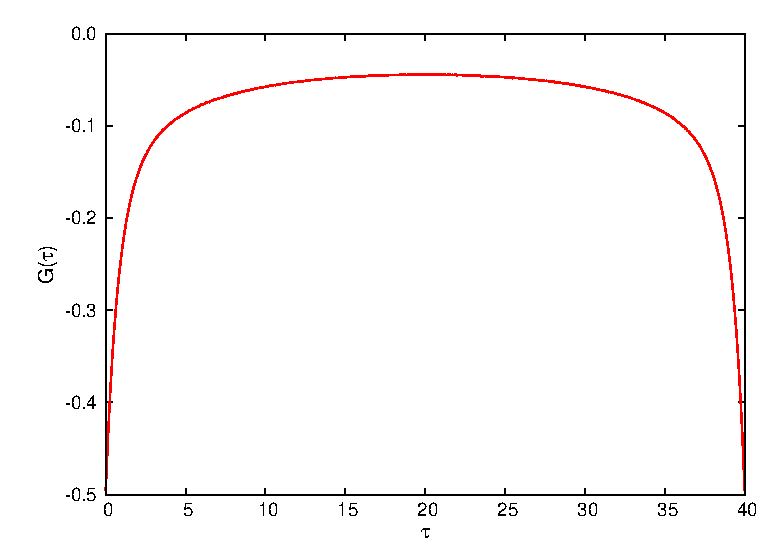
\includegraphics{figure/green.eps}
\caption{单带半满Hubbard模型的虚时格林函数$G(\tau)$} 
\label{fig:green}
\end{figure}

图\ref{fig:green}中给出的是虚时格林函数$G(\tau)$,用户首先要检查该函数
曲线是否足够光滑,尤其是底部靠近0的位置是否光滑。有一个经验是,如果底
部非常贴近0\footnote{所谓的底部指的是$\tau = \beta/2$附近两侧的地方。},
那么该系统是绝缘相。图\ref{fig:green}清楚地表明系统属于典型的金属相。
除此之外,还需确认所有的$G(\tau)$数据点均小于0,如果大于0则是不合理的。

\begin{figure}
\centering
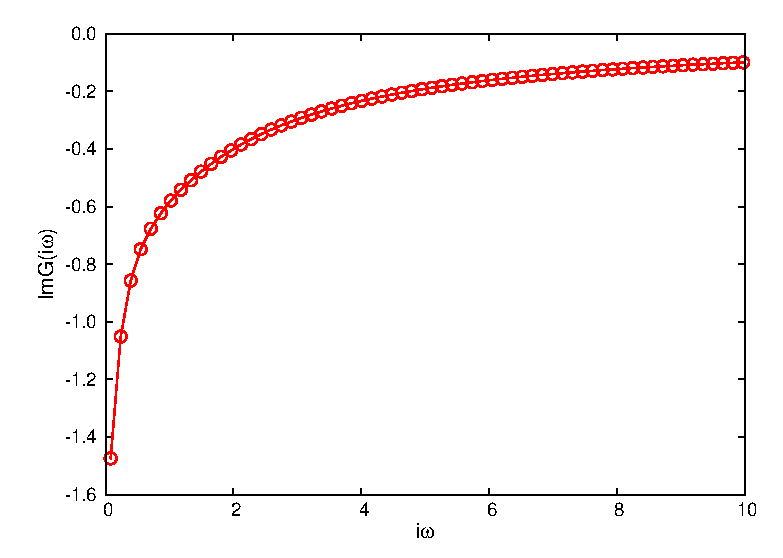
\includegraphics{figure/grn.eps}
\caption{单带半满Hubbard模型的虚频格林函数的虚部$\Im G(i\omega)$} 
\label{fig:grnim}
\end{figure}

图\ref{fig:grnim}中给出的是虚频格林函数的虚部$\Im G(i\omega)$,仅仅画
出了低频部分的数据点。用户也需要检查该函数曲线是否足够光滑,尤其是随
着频率增大$\omega \rightarrow \infty$,曲线应该有趋近于0的渐进行为。
$\Im G(i\omega)$的低频部分的弯曲情况可以用来粗略判断系统处在什么相。
如果是一个勾($\surd$)的形状,那么该系统应该处于绝缘相,反之,则属于
金属相。图\ref{fig:grnim}明显展示的是金属相的特征,与上文的推测相符。

\begin{figure}
\centering
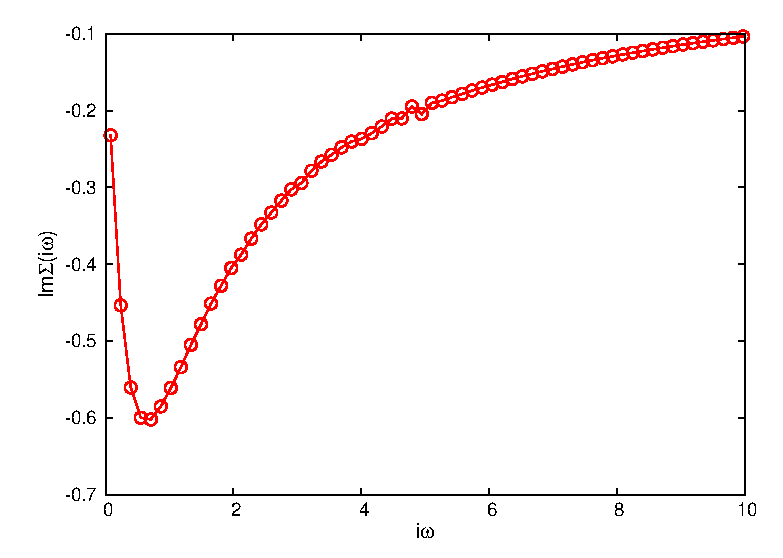
\includegraphics{figure/sgm.eps}
\caption{单带半满Hubbard模型的电子自能函数的虚部$\Im \Sigma(i\omega)$} 
\label{fig:sgmim}
\end{figure}

图\ref{fig:sgmim}中给出的是虚频电子自能函数的虚部$\Im \Sigma(i\omega)$,
仅仅画出了低频部分的数据点。用户也需要检查该函数曲线是否足够光滑,尤其
是随着频率增大$\omega \rightarrow \infty$,曲线应该有趋近于0的渐进行为。

D:分析$P_{\text{H}}$、$P_{\Gamma}$数据

\begin{figure}
\centering
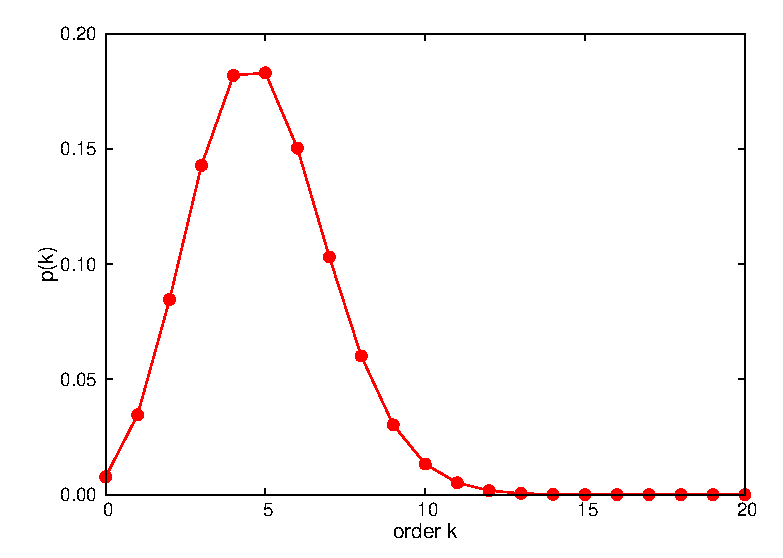
\includegraphics{figure/hist.eps}
\caption{图形微扰展开序列的阶数分布$P_{\text{H}}$} 
\label{fig:hist}
\end{figure}

图形微扰展开序列的阶数分布$P_{\text{H}}$以及原子组态的概率分布$P_{\Gamma}$
能提供十分重要的信息。

使用如下命令可以绘制出$P_{\text{H}}$数据:

\noindent\colorbox{pink}{\parbox[r]{\linewidth}{\quad \$ gnuplot> plot [0:20] "solver.hist.dat" u 1:3 w lp }}

请注意,0阶的数据是位于文件最后的一行,请在绘图之前将最后一行剪切粘贴到
1阶那一行之前,并把阶数由1024改为0(参见第\ref{sec:hist}小节)。
图\ref{fig:hist}给出的是本次计算所获得的图型微扰展开阶数的分布情况。不难
发现,图中曲线是以5为中心的类Gaussian分布。由此,我们可以得到一个直观
的认识:那就是在应用连续时间量子蒙特卡洛算法进行抽样时,高阶项和低阶项的
出现概率是非常低的,因此计算结果不会出现发散。

另外用户也可以用vim查看solver.prob.dat文件,了解原子组态概率的分布情
况$P_{\Gamma}$。在本例中,应该是单占据态($N = 1$)的出现概率占据了绝
大部分,空占据态($N = 0$)以及双占据态($N = 2$)的出现概率比较小。

OK!到目前为止你已经完成了第一个例子:使用{\iqist}软件包的{\azalea}量子
杂质求解器组件在动力学平均场理论的框架内求解了一个单带半满Hubbard模型。
这个例子十分简单,但是却十分的重要,由此学到的方法和技巧将会帮助你挑战
更困难的问题。

\subsection{Mott金属$-$绝缘体相变}
\label{subsec:mott}

在本案例中,主要展示如何应用{\iqist}软件包来研究Mott金属$-$绝缘体相变。
研究对象还是最简单的bethe晶格上的单带半满Hubabrd模型,此模型已经包含了
Mott金属$-$绝缘体相变现象的绝大部分物理在内。众所周知,Mott相变的主要
驱动力是Coulomb相互作用$U$,因此我们只需在上一个案例的基础上,调整
solver.ctqmc.in输入文件中$U$参数的值,再重复进行几次DMFT自洽计算即可。事
不宜迟,下面让我们按部就班开始计算吧。

步骤1:\underline{创建自己的工作目录/工作文件夹}

首先创建iqist\_test文件夹,该文件夹可作为用户的练习目录。如果用户在练
习上一个案例时已经创建了此文件夹,那么可以略过此操作。

在iqist\_test文件夹下创建子文件夹t812:

\noindent\colorbox{pink}{\parbox[r]{\linewidth}{\quad \$ mkdir t812 }}

再进入到t812文件夹中:

\noindent\colorbox{pink}{\parbox[r]{\linewidth}{\quad \$ cd t812 }}

那么当前所在的位置就是/iqist\_test/t812。

我们选择9组不同的$U$值进行计算,分别为:1.0、1.5、2.0、2.5、3.0、3.5、
4.0、5.0、6.0 eV。请为不同的$U$值建立相应的文件夹,分别为u10、u15、
u20、u25、u30、u35、u40、u50、u60。创建文件夹的命令示例如下:

\noindent\colorbox{pink}{\parbox[r]{\linewidth}{\quad \$ mkdir u10 u15 u20 u25 u30 u35 u40 u50 u60}}

步骤2:\underline{准备solver.ctqmc.in}

在/opt/iqist/tutor/t812文件夹中,我们已经准备好了{\azalea}组件的输
入文件solver.ctqmc.in,请将它复制到当前目录下对应的文件夹中,例如:

\noindent\colorbox{pink}{\parbox[r]{\linewidth}{\quad \$ cp /opt/iqist/tutor/t812/u10/solver.ctqmc.in ./u10 }}

u10/solver.ctqmc.in文件与u20/solver.ctqmc.in文件基本上完全一致,差
别仅在于$U$、$U_{c}$、$U_{v}$与mune参数的设置。用户可以使
用diff/colordiff命令比较这两个文件的异同。

\noindent\colorbox{pink}{\parbox[r]{\linewidth}{\quad \$ diff u10/solver.ctqmc.in u20/solver.ctqmc.in }}

用户可进一步两两比较其它文件夹中的solver.ctqmc.in文件,亦能得到类似的发现。

步骤3:\underline{启动{\azalea}组件进行实际计算}

依次进入到各个u*文件夹中,按照上一小节介绍的方法,启动{\azalea}组件
的ctqmc程序进行计算。完成全部计算过程估计需要一段时间,用户可以利用
这段时间来阅读该文档的其它部分内容。

步骤4:\underline{数据的分析和处理}

\begin{figure}
\centering
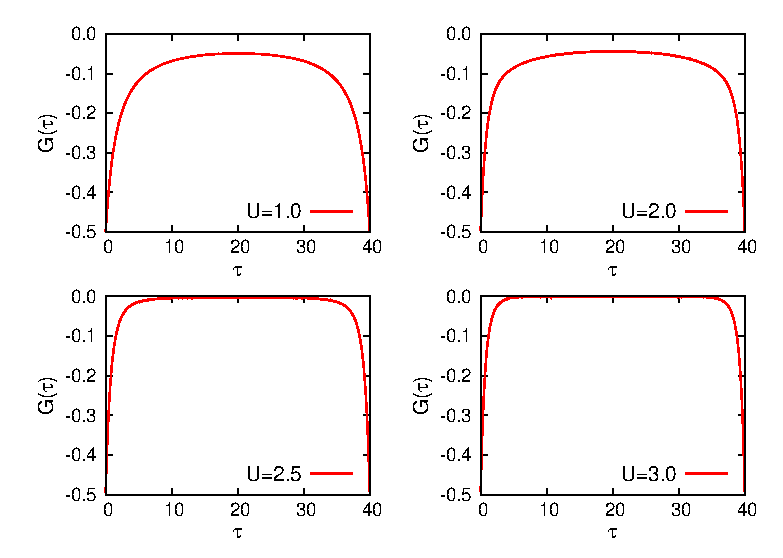
\includegraphics{figure/green-mit.eps}
\caption{虚时格林函数$G(\tau)$随着$U$的变化} 
\label{fig:green-mit}
\end{figure}

\begin{figure}
\centering
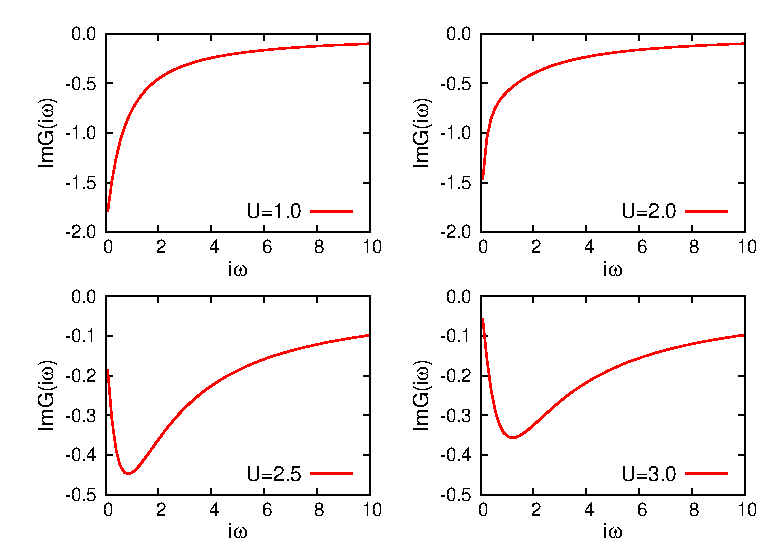
\includegraphics{figure/grn-mit.eps}
\caption{虚频格林函数的虚部$\Im G(i\omega)$随着$U$的变化} 
\label{fig:grnim-mit}
\end{figure}

\begin{figure}
\centering
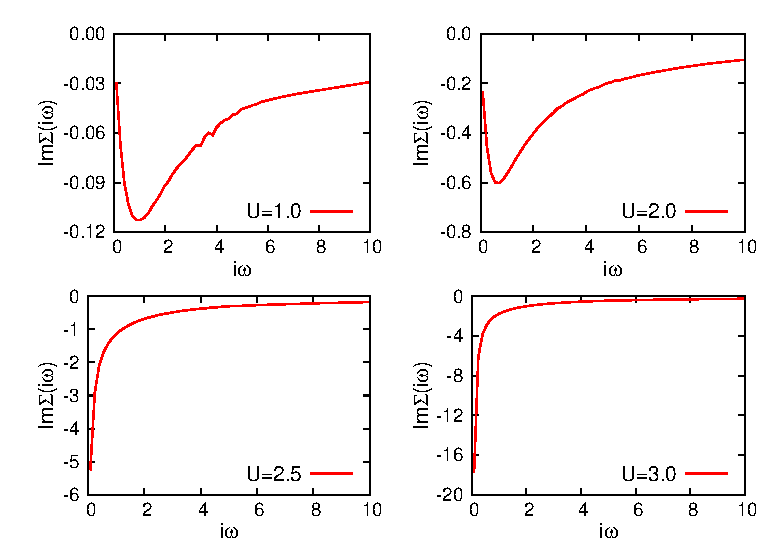
\includegraphics{figure/sgm-mit.eps}
\caption{电子自能函数的虚部$\Im \Sigma (i\omega)$随着$U$的变化} 
\label{fig:sgmim-mit}
\end{figure}

\begin{figure}
\centering
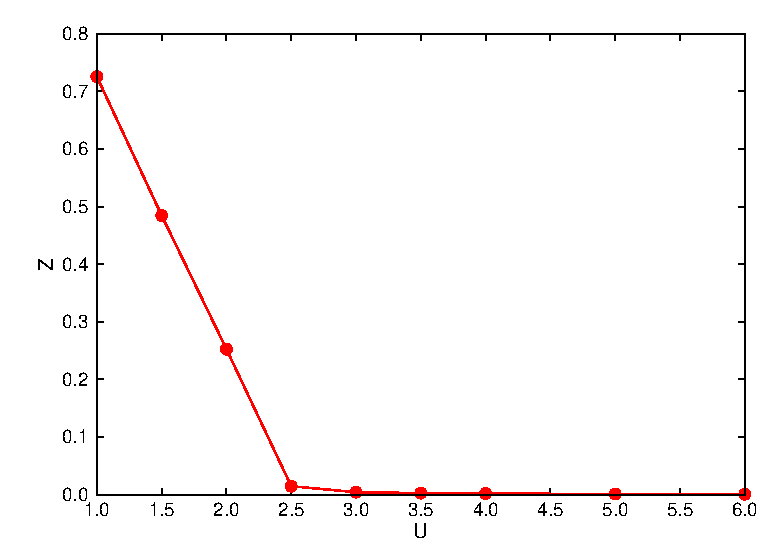
\includegraphics{figure/quasi.eps}
\caption{准粒子权重$Z$随着$U$的变化} 
\label{fig:quasi-mit}
\end{figure}

\begin{figure}
\centering
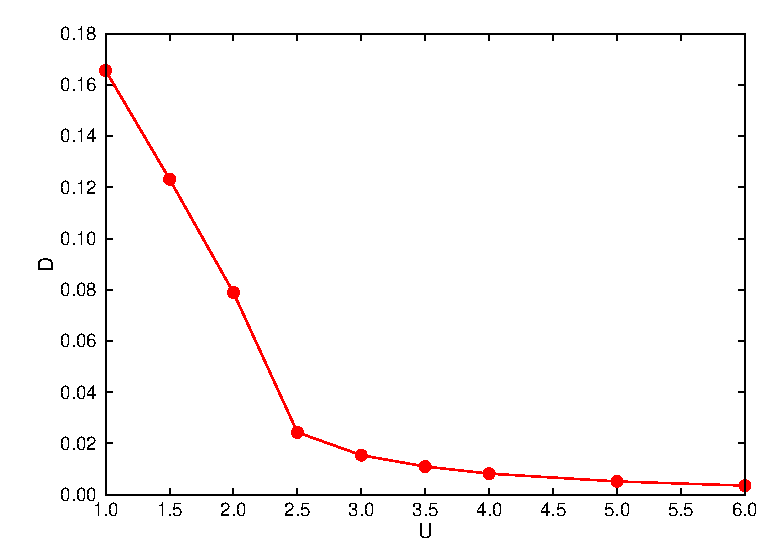
\includegraphics{figure/double.eps}
\caption{双占据数$D$随着$U$的变化} 
\label{fig:double-mit}
\end{figure}

\begin{figure}
\centering
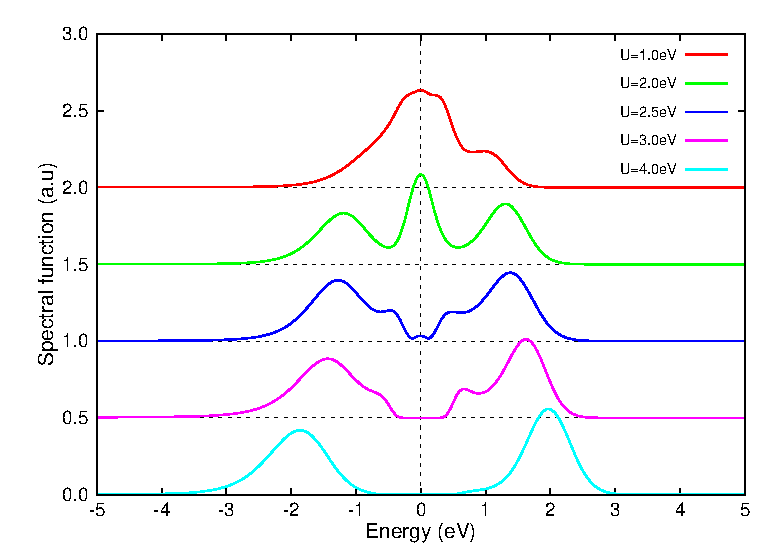
\includegraphics{figure/spec.eps}
\caption{单粒子谱函数$A(\omega)$随着$U$的变化} 
\label{fig:A-mit}
\end{figure}

当所有$U$值的DMFT计算都进行完毕之后,我们需要对计算结果进行细致的分析,以判明是
否发生了Mott金属$-$绝缘体相变。请首先检查每个u*文件夹的out.dat文件,确认该次计算
没有异常出现。接下来先选取几个典型的$U$值,用gnuplot画出相应的虚时格林函数$G(\tau)$
(参见图\ref{fig:green-mit})、虚频格林函数的虚部$\Im G(i\omega)$(参见
图\ref{fig:grnim-mit})与虚频电子自能函数的虚部$\Im \Sigma(i\omega)$(参见
图\ref{fig:sgmim-mit})。通过细致比较这几个图,用户可以看到随着$U$的逐渐增
大,体系是如何从金属相转变到Mott绝缘相的。很明显,当$U$ = 2.0\ eV时,系统
还处于金属相,但是当$U$ = 2.5\ eV时,系统已经转化为绝缘相。

对于Mott金属$-$绝缘体转变,准粒子权重$Z$最能准确地反应相变的进程。$Z$为大于0的有限
值意味着金属相,$Z$接近于0意味着Mott绝缘相。我们可以利用一个近似公式来计算准粒子权
重$Z$,该公式如下所示:
\begin{equation}
Z \approx \frac{1}{1-\frac{\Im \Sigma(i\omega_{0})}{\omega_{0}}}
\end{equation}
其中,$\Im \Sigma(i\omega_{0})$是虚频电子自能函数的虚部在第一个频率点上的值,
$\omega_{0}$是第一个松原频率点。该公式在温度$T = 0$\ K时严格成立,当温度很低时仍
是一个很好的近似。如图\ref{fig:quasi-mit}所示,随着Coulomb相互作用$U$的增大,准粒
子权重$Z$不断下降,最后趋近于0,体系从金属变为Mott绝缘体。此相变的相变点大致位于
$U \sim$ 2 - 2.5\ eV。另外一个反映相变过程的关键物理量为双占据数。在上一个案例中
我们已经介绍了如何得到双占据数,此刻将双占据数对$U$作图,如图\ref{fig:double-mit}
所示。不难发现,双占据数和准粒子权重具有类似的变化趋势,这反应了电子在逐渐增强的
Coulomb相互作用下,从巡游态变为局域态。

最后,我们可以将虚时格林函数$G(\tau)$进行解析延拓(请参阅
第\ref{subsec:ac-g}小节),得到电子谱函数$A(\omega)$。如图\ref{fig:A-mit}所
示,增大$U$值时,电子谱函数从近自由电子形状演化到具有三峰结构。继续增大$U$,
谱函数将打开能隙,表明体系进入到Mott绝缘体相。

\section{进阶应用I:新的物理}
\label{sec:stage1}

在上一节,我们所介绍的案例均是基于半满的单带Hubbard模型,其所包含的物理比较简
单。在这一节,我们将以多带模型为例,进一步向用户展示{\iqist}软件包的强大功能。
多带模型蕴涵了许多新的物理,这是{\iqist}软件包的主要战场之所在。

\subsection{广义相互作用项}
\label{subsec:general}

利用{\azalea}组件可对具有密度$-$密度相互作用的Hubbard模型进行了研究,但是对于具有
广义相互作用项的多带Hubbard模型,基于段表示算法的{\azalea}组件就不再适用了。在本小
节,我们将展示如何使用基于广义矩阵算法的{\begonia}组件来研究bethe晶格上的两带半满
Hubbard模型。

该两带Hubbard模型的局域哈密顿量如下:
\begin{equation}
\label{eq:loc}
\begin{split}
H_{loc} = &- \sum_{a\sigma}(\mu - \Delta_a) n_{a\sigma} + \sum_{a} Un_{a\uparrow}n_{a\downarrow} \\
          &+ \sum_{a > b,\sigma}[U'n_{a\sigma}n_{b\bar{\sigma}} + (U'-J)n_{a\sigma}n_{b\sigma}] \\
          &- \sum_{a < b} J (d^{\dagger}_{a\downarrow}d^{\dagger}_{b\uparrow}d_{b\downarrow}d_{a\uparrow} 
           + d^{\dagger}_{b\uparrow}d^{\dagger}_{b\downarrow}d_{a\uparrow}d_{a\downarrow} + h.c.).
\end{split}
\end{equation}
其中,$a$,$b$为能带指标($a, b = 1 \sim 2$),$\sigma$为自旋指标,$n_{a\sigma} = 
c^{\dagger}_{a\sigma}c_{a\sigma}$为占据数算符,$\mu$为化学势,$U$($U'$)分
别为轨道间(轨道内)Coulomb相互作用,$\Delta$为杂质能级\footnote{在本案例中
$\Delta = 0$。}。上式右端的第三项为自旋$-$翻转项与对跃迁项,如果哈密顿量
包含了这一项,我们就称此相互作用是广义的,具有旋转不变性,如果没有这一项,
那么此相互作用具有密度$-$密度形式。在本案例中,假定$J = J_{z} = J_{s} = J_{p}$,
也就说,此两带模型具有广义形式的相互作用项。对于此类型的哈密顿量,必须使
用基于广义矩阵算法的量子杂质求解器组件,例如{\begonia}组件或者是{\lavender}
组件来进行求解。下面我们展示如何使用最简单的{\begonia}组件来求解此两带模
型,具体计算流程如下。

步骤1:\underline{创建自己的工作目录/工作文件夹}

首先创建iqist\_test文件夹,该文件夹可作为用户的练习目录。如果用户在练习上
一个案例时已经创建了此文件夹,那么可以略过此操作。

在iqist\_test文件夹下创建子文件夹t821:

\noindent\colorbox{pink}{\parbox[r]{\linewidth}{\quad \$ mkdir t821 }}

再进入到t821文件夹中:

\noindent\colorbox{pink}{\parbox[r]{\linewidth}{\quad \$ cd t821 }}

那么当前所在的位置就是/iqist\_test/t821。

步骤2:\underline{准备solver.ctqmc.in}

在/opt/iqist/tutor/t821文件夹中,我们已经准备好了{\begonia}组件的输入
文件solver.ctqmc.in,请将它复制到当前目录下,例如:

\noindent\colorbox{pink}{\parbox[r]{\linewidth}{\quad \$ cp /opt/iqist/tutor/t821/solver.ctqmc.in . }}

关于{\begonia}组件的solver.ctqmc.in输入文件,用户要注意以下几点:
\begin{itemize}
  \item 此时$U$、$U_{c}$、$U_{v}$、$J_{z}$、$J_{s}$与$J_{p}$等参数是无效
        的,因为相关参数已经在原子问题程序{\jasmine}组件(请参阅
        第\ref{sec:jasmine}节)里设定了,所以从原则
        上说这些值设不设都无所谓。但是为了方便事后复查计算过程,我们建议
        用户还是正确设定上述参数。
  \item 化学势mune设为3.954869,此时占据数为半满。
  \item npart参数的最佳取值不好确定,建议设为1,这是最稳妥的数值,但是计
        算效率未必是最佳的。关于npart参数的详情,请参阅第\ref{sec:part}节。
\end{itemize}

步骤3:\underline{准备atom.in}

在/opt/iqist/tutor/t821文件夹中,我们已经准备好了{\jasmine}组件的输入文
件atom.in,请将它复制到当前目录下,例如:

\noindent\colorbox{pink}{\parbox[r]{\linewidth}{\quad \$ cp /opt/iqist/tutor/t821/atom.in . }}

在该文件中,主要设定了如下参数
\begin{itemize}
\item $U=U_{c}=4.0$
\item $J_{z}=J_{s}=J_{p}=0.25U=1.0$
\item $U_{v}=U_{c}-2J_{z}=2.0$
\item isoce = -1
\item lsoc = 0.0
\item eimp = 0.0
\end{itemize}
至于atom.in输入文件的其它参数项,请查看输入文件中的注释以及第\ref{sec:jasmine}
节对于输入参数的解释。

步骤4:\underline{运行{\jasmine}组件程序}

利用{\jasmine}组件来对角化原子问题,直接执行如下命令:

\noindent\colorbox{pink}{\parbox[r]{\linewidth}{\quad \$ atom }}

该程序很快执行完毕,如果没有输出任何错误信息的话,这表示用户的计算已经成
功了。在当前目录中将会出现很多以atom打头的数据文件,其中唯有atom.cix是最
重要的,它是基于广义矩阵算法的量子杂质求解器组件必须的输入文件(请参阅
第\ref{sec:ac}节),缺失该文件将导致{\begonia}程序不能运行。

步骤5:\underline{启动{\begonia}组件进行实际计算}

在此案例中,我们使用8个计算核心运行{\begonia}组件的ctqmc程序,用户可以根
据现有的计算资源做出适当调整。具体命令如下:

\noindent\colorbox{pink}{\parbox[r]{\linewidth}{\quad \$ nohup mpiexec -n 8 ctqmc < /dev/null >  out.dat \&}}
{\begonia}组件程序所须的运行时间较长,请用户耐心等待。

步骤6:\underline{监测{\begonia}组件的运行状态}

密切观察ctqmc程序的运行情况,在第一时间内对异常情况做出反应十分必要。
用户需要不时查看输出文件out.dat,关注的信息除了
前面章节所提到的以外,用户还需要额外关注的是Monte Carlo抽样算法符号问题
的统计信息,如下所示\footnote{请注意:{\azalea}、{\gardenia}与{\narcissus}
组件是不会输出如下统计信息的,因为在这些组件中不存在负符号问题\cite{yoo:10307}。}:
\begin{lstlisting}[frame=single]
    negative sign counter:         0
    averaged sign sampler:   1.00000
\end{lstlisting}
其中第1行是抽样时负符号出现的次数,第2行是正符号和负符号的平均值。如果
该平均值的绝对值趋于0,那么表示正号和负号各占一半,符号问题最严重了,
此时Monte Carlo抽样结果完全是不可信的。在我们研究的这个模型中,几乎
没有负符号出现,因此计算是可信的。

步骤7:\underline{数据的分析和处理}

\begin{figure}
\centering
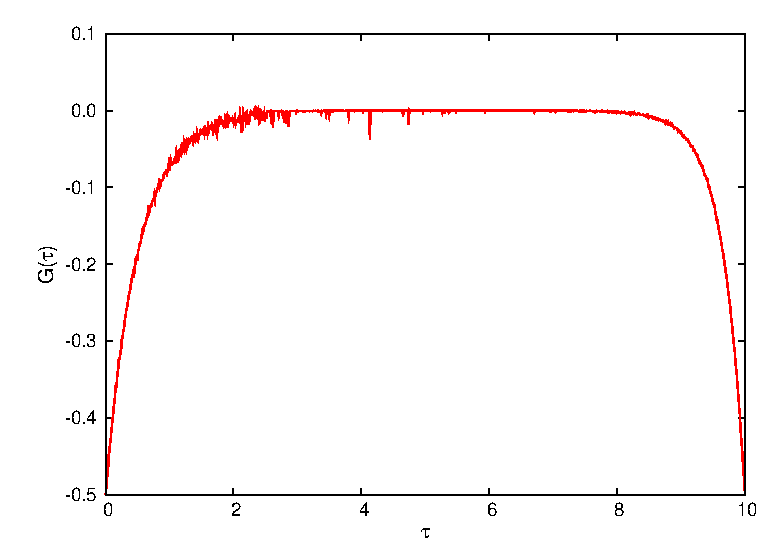
\includegraphics{figure/green-t821.eps}
\caption{广义相互作用的两带半满Hubbard模型的虚时格林函数$G(\tau)$} 
\label{fig:green-t821}
\end{figure}

\begin{figure}
\centering
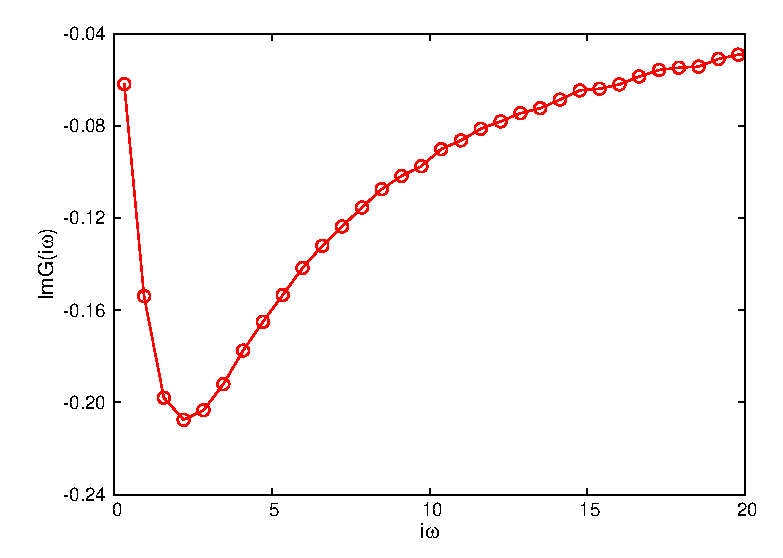
\includegraphics{figure/grn-t821.eps}
\caption{广义相互作用的两带半满Hubbard模型的虚频格林函数的虚部$\Im G(i\omega)$} 
\label{fig:grn-t821}
\end{figure}

\begin{figure}
\centering
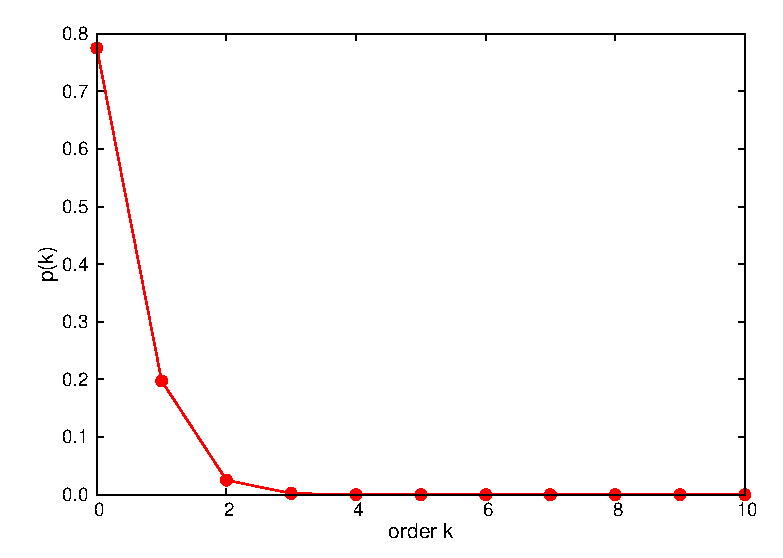
\includegraphics{figure/hist-t821.eps}
\caption{广义相互作用的两带半满Hubbard模型的图形微扰展开序列的阶数分布$P_{\text{H}}$} 
\label{fig:hist-t821}
\end{figure}

确认计算完成后,用户可以按照上一节中介绍的方法分析计算结果。在这里
分析任务就交给用户自己去完成了。我们计算结果如下: 图\ref{fig:green-t821}
展示的是虚时格林函数$G(\tau)$,图\ref{fig:grn-t821}展示的是虚频格
林函数的虚部$\Im G(i\omega)$,图\ref{fig:hist-t821}展示的是图形微
扰展开序列的阶数分布$P_{\text{H}}$。原子组态概率如下所示:

\begin{lstlisting}[frame=single]
# state probability: index | prob | occupy | spin
    1    0.000017    0.000000    0.000000
    2    0.002528    1.000000    0.500000
    3    0.002514    1.000000    0.500000
    4    0.002538    1.000000   -0.500000
    5    0.002557    1.000000   -0.500000
    6    0.326522    2.000000    1.000000
    7    0.326595    2.000000    0.000000
    8    0.326408    2.000000   -1.000000
    9    0.000057    2.000000    0.000000
   10    0.000054    2.000000    0.000000
   11    0.000035    2.000000    0.000000
   12    0.002546    3.000000    0.500000
   13    0.002559    3.000000    0.500000
   14    0.002537    3.000000   -0.500000
   15    0.002510    3.000000   -0.500000
   16    0.000022    4.000000    0.000000
\end{lstlisting}

\subsection{自旋$-$轨道耦合作用}
\label{subsec:soc}

在本小节,我们将引导用户使用{\iqist}软件包来研究含自旋$-$轨道耦合项的系统。
对于重元素体系,尤其是$4f/5f$电子系统而言,自旋$-$轨道耦合效应起着十分重
要的作用,它与Coulomb相互作用之间存在着相互竞争的关系,这也是最近凝聚态物
理领域十分热门的研究课题。此次我们的研究对象是一个定义在bethe晶格上的三带
Hubbard模型,该模型不但具有广义相互作用项(参见公式(\ref{eq:loc})),并且还具
有自旋$-$轨道耦合项。自旋$-$轨道耦合项的哈密顿量如下所示:

\begin{equation}
\label{eqn:soc}
H_{soc}=\sum_{a\sigma,b\sigma^{\prime}} \zeta 
\langle a\sigma | l_{x}s_{x} + l_{y}s_{y} + l_{z}s_{z} | b\sigma^{\prime} \rangle 
d_{a\sigma}^{\dagger}d_{b\sigma^{\prime}}
\end{equation}

其中$\zeta$为自旋$-$轨道耦合作用强度。在{\iqist}软件包中,唯有定制的{\lavender}
组件\footnote{标准版的{\lavender}组件不可用于此类计算。}可以求解此模型哈密
顿量。具体的计算步骤如下。

步骤1:\underline{创建自己的工作目录/工作文件夹}

首先创建iqist\_test文件夹,该文件夹可作为用户的练习目录。如果用户在练习上
一个案例时已经创建了此文件夹,那么可以略过此操作。

在iqist\_test文件夹下创建子文件夹t822:

\noindent\colorbox{pink}{\parbox[r]{\linewidth}{\quad \$ mkdir t822 }}

再进入到t822文件夹中:

\noindent\colorbox{pink}{\parbox[r]{\linewidth}{\quad \$ cd t822 }}

那么当前所在的位置就是/iqist\_test/t822。

步骤2:\underline{准备solver.ctqmc.in}

在/opt/iqist/tutor/t822文件夹中,我们已经准备好了{\lavender}组件的输入文
件solver.ctqmc.in,请将它复制到当前目录下,例如:

\noindent\colorbox{pink}{\parbox[r]{\linewidth}{\quad \$ cp /opt/iqist/tutor/t822/solver.ctqmc.in . }}

关于{\lavender}组件的solver.ctqmc.in输入文件,用户要注意以下几点:
\begin{itemize}
  \item 由于有自旋$-$轨道耦合项,$S_{z}$不再是好量子数,需要设置
        isspn = 2,issun = 2。
  \item 使用Legendre正交多项式方法测量虚时格林函数,设置isort = 2,这
        样可以得到比较平滑的虚时格林函数$G(\tau)$。
  \item 此时$U$、$U_{c}$、$U_{v}$、$J_{z}$、$J_{s}$与$J_{p}$参数是无效
        的,因为相关参数已经在原子问题程序里设定好了,所以从原则上说这
        些值设不设都无所谓。但是为了方便事后复查计算过程,我们建议用户
        还是正确设定上述参数。
  \item 化学势mune设为8.360310,此时总占据数恰好为4.0。
  \item 设置Legendre正交多项式的最大展开阶数lemax = 24。
  \item 设置Legendre正交多项式线性网格点数目legrd = 20001。
  \item 关闭GLOBAL FLIP更新操作,设置nflip = 0。
\end{itemize}

步骤3:\underline{准备solver.eimp.in}

在/opt/iqist/tutor/t822文件夹中,我们已经准备好了{\lavender}组件的输入
文件solver.eimp.in,请将它复制到当前目录下,例如:

\noindent\colorbox{pink}{\parbox[r]{\linewidth}{\quad \$ cp /opt/iqist/tutor/t822/solver.eimp.in . }}

在该文件中,我们设定杂质能级都为0.0,前4个轨道兼并,对应$j = 3/2$态,
后2个轨道兼并,对应$j = 1/2$态。{\lavender}组件将利用这些设置对轨道
进行强制对称化(issun = 2)。

步骤4:\underline{准备dft.atom.in}

由于{\jasmine}组件目前尚不支持自旋$-$轨道耦合作用,因此我们无法再利
用它来对角化原子问题,以产生atom.cix文件,详情请参阅第\ref{sec:jasmine}
节。十分幸运的是,杜亮博士为他的原子问题程序rambutan针对{\lavender}组件
开发了专用的接口,我们可以使用他的程序来产生atom.cix文件。
rambutan程序所需要的输入文件为dft.atom.in。在/opt/iqist/tutor/t822文件
夹中,我们已经准备好了dft.atom.in文件,请将它复制到当前目录下,例如:

\noindent\colorbox{pink}{\parbox[r]{\linewidth}{\quad \$ cp /opt/iqist/tutor/t822/dft.atom.in . }}

在dft.atom.in文件中,主要设定了以下参数:

\begin{itemize}
\item $U = U_{c} = 4.0$
\item $J_{z} = J_{s} = J_{p} = 0.25U = 1.0$
\item $U_{v} = U_{c} - 2J_{z} = 2.0$
\item $\zeta=-0.20$\footnote{此为rambutan程序中定义的自旋$-$轨道耦合
      强度,请注意它采用了负号规范。}
\end{itemize}
至于dft.atom.in输入文件的其它设置参数,请用户仔细查看输入文件中的注释或者
是直接向杜亮博士咨询(mailto:duliang@iphy.ac.cn)。

步骤5:\underline{运行rambutan程序}

运行rambutan程序来对角化原子问题,rambutan的可执行程序名为atomic,使用
如下命令:

\noindent\colorbox{pink}{\parbox[r]{\linewidth}{\quad \$ atomic }}

该程序很快执行完毕,如果没有输出任何错误信息的话,表示用户的计算很成功,
rambutan程序产生了标准的atom.cix文件。此文件是基于广义矩阵算法的量子杂
质模型求解器所必须的输入文件(请参阅第\ref{sec:ac}节),缺失该文件将导
致{\lavender}组件的ctqmc程序不能运行。

步骤6:\underline{启动{\lavender}组件进行实际计算}

在此案例中,我们使用8个计算核心运行{\lavender}组件的ctqmc程序,用户可以根据现
有的计算资源做出适当调整。具体命令如下:

\noindent\colorbox{pink}{\parbox[r]{\linewidth}{\quad \$ nohup mpiexec -n 8 ctqmc < /dev/null >  out.dat \&}}
{\lavender}组件程序所须的运行时间较长,请用户耐心等待。

步骤7:\underline{监测{\lavender}组件的运行状态}

密切观察ctqmc程序的运行情况,在第一时间内对异常情况做出反应十分必要。
用户需要不时查看输出文件out.dat,关注的信息除了前面章节所提
到的以外,用户还需要额外关注的是Monte Carlo抽样算法符号问题
的统计信息,如下所示\footnote{{\begonia}、{\lavender}、{\camellia}、
{\epiphyllum}、{\pansy}与{\manjushaka}等基于广义矩阵算法的
量子杂质求解器组件均会输出与负符号问题有关的统计信息。}:
\begin{lstlisting}[frame=single]
    negative sign counter:   3802766
    averaged sign sampler:   0.61972
\end{lstlisting}
其中第1行是抽样时负符号出现的次数,第2行是正符号和负符号的平均值。如
果该平均值的绝对值趋于0,那么表示正号和负号各占一半,符号问题最严重
了,此时Monte Carlo抽样结果完全是不可信的。在我们研究的这个模型中,
有负符号出现,但是负符号问题还不是十分严重,计算结果还是基本可信的。

步骤8:\underline{数据的分析和处理}

\begin{figure}
\centering
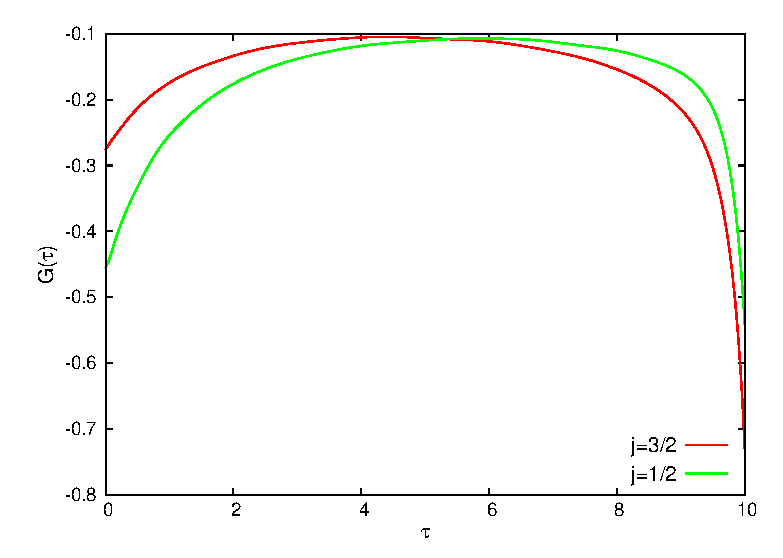
\includegraphics{figure/green-t822.eps}
\caption{包含自旋$-$轨道耦合的三带Hubbard模型的虚时格林函数$G(\tau)$} 
\label{fig:green-t822}
\end{figure}

\begin{figure}
\centering
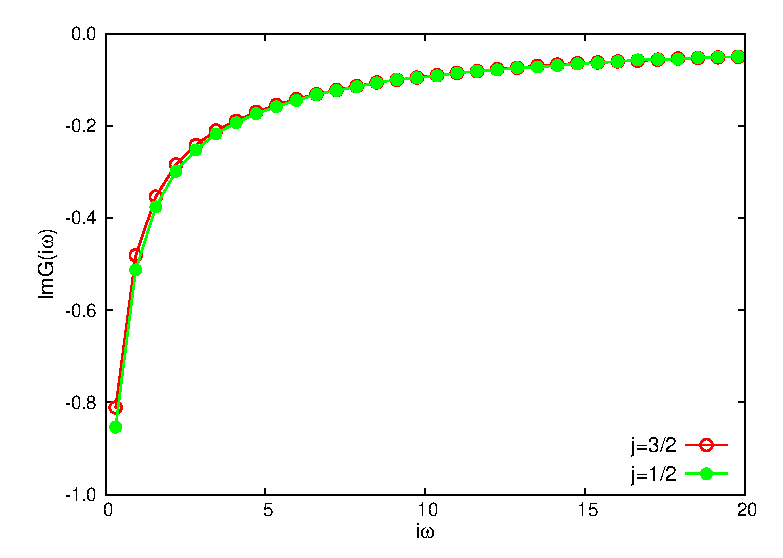
\includegraphics{figure/grn-t822.eps}
\caption{包含自旋$-$轨道耦合的三带Hubbard模型的虚频格林函数的虚部$\Im G(i\omega)$} 
\label{fig:grn-t822}
\end{figure}

\begin{figure}
\centering
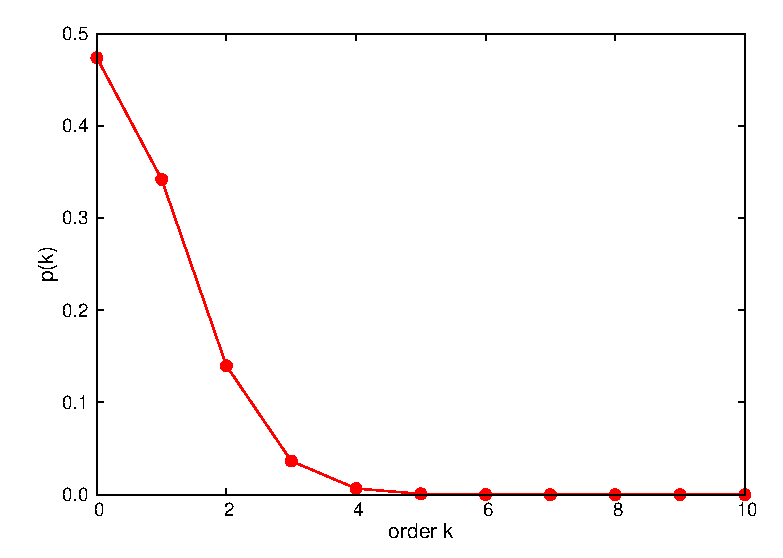
\includegraphics{figure/hist-t822.eps}
\caption{包含自旋$-$轨道耦合的三带Hubbard模型的图形微扰展开序列的阶数分布$P_{\text{H}}$} 
\label{fig:hist-t822}
\end{figure}

在漫长的等待过后,计算终于成功结束了。在确认计算完成后,用户可以按照
第\ref{sec:basic}节中介绍的方法分析计算结果。在这里分析任务就交给用户
自己去完成了。我们计算结果如下: 图\ref{fig:green-t822}展示的是
虚时格林函数$G(\tau)$,由于采用了Legendre正交多项式方法测量$G(\tau)$,
因此$G(\tau)$函数的曲线显得尤为平滑;图\ref{fig:grn-t822}展示的是虚频格林函数
的虚部$\Im G(i\omega)$,显而易见,自旋$-$轨道耦合效应导致原来简并
的三条能带发生了劈裂;图\ref{fig:hist-t822}展示的是图形微扰展
开序列的阶数分布$P_{\text{H}}$。占据数情况如下:

\begin{itemize}
\item $j=3/2$轨道,平均占据数为0.728540
\item $j=1/2$轨道,平均占据数为0.542734
\end{itemize}

用户还可以变换Coulomb相互作用强度$U$以及自旋$-$轨道耦合作用强度$\zeta$,
重复进行上述计算,深入探讨自旋$-$轨道耦合作用对于关联电子系统电子结构
的影响\footnote{相关的研究结果可以参阅{\color{red}arXiv:1211.2055}。}。

\subsection{晶体场劈裂效应}
\label{subsec:cfs}

在本小节中我们将利用{\iqist}软件包来研究多带Hubbard模型中的晶体场劈裂
效应。我们的研究对象是bethe晶格上的两带Hubbard模型,晶体场将使两个
能带发生劈裂。为了简化问题,此处暂不考虑广义相互作用,仅仅考虑密度
$-$密度形式的相互作用。这样我们就可以利用高效的{\azalea}组件来解决
问题。

步骤1:\underline{创建自己的工作目录/工作文件夹}

首先创建iqist\_test文件夹,该文件夹可作为用户的练习目录。如果用户在
练习上一个案例时已经创建了此文件夹,那么可以略过此操作。

在iqist\_test文件夹下创建子文件夹t823:

\noindent\colorbox{pink}{\parbox[r]{\linewidth}{\quad \$ mkdir t823 }}

再进入到t823文件夹中:

\noindent\colorbox{pink}{\parbox[r]{\linewidth}{\quad \$ cd t823 }}

那么当前所在的位置就是/iqist\_test/t823。

步骤2:\underline{准备solver.ctqmc.in}

在/opt/iqist/tutor/t823文件夹中,我们已经准备好了{\azalea}组件的输入
文件solver.ctqmc.in,请将它复制到当前目录下,例如:

\noindent\colorbox{pink}{\parbox[r]{\linewidth}{\quad \$ cp /opt/iqist/tutor/t823/solver.ctqmc.in . }}

此solver.ctqmc.in文件的关键设置如下:
\begin{itemize}
  \item 采用自洽计算模式,isscf = 2
  \item 强制进行轨道对称化处理,issun = 2
  \item 强制进行自旋对称化处理,isspn = 1
  \item 该模型有2条能带,nband = 2
  \item 自旋投影方向,nspin = 2
  \item 轨道数目,norbs = 4
  \item 原子组态数目,ncfgs = 16
  \item 最大DMFT自洽迭代次数,niter = 20
  \item 库仑相互作用强度,$U$ = $U_{c}$ = 4.0,$U_{v}$ = $U_{c}-2J_{z}$ = 2.0 
  \item Hund交换作用强度,$J_{z}$ = $0.25U$ = 1.0,$J_{s}$ = $J_{p}$ = 0.0
  \item 化学势,mune = 2.0
  \item 反温度,beta = 10.0
  \item 最近邻跃迁系数,part = 0.50
\end{itemize}
上述设置与不存在晶体场劈裂时的情况基本一致,没有什么特别之处。

步骤3:\underline{准备solver.eimp.in}

各轨道的杂质能级必须在solver.eimp.in文件中设定。在默认情况下,杂质能级都是
0.0,所有轨道完全简并,因此可以不提供solver.eimp.in文件给量子杂质求解器组
件作为输入。但是在本案例中,各轨道的杂质能级不再为0.0,轨道之间存在着晶体
场劈裂,因此solver.eimp.in文件是必须的(关于solver.eimp.in文件的细节,请参
阅第\ref{sec:sei}节)。

在/opt/iqist/tutor/t823文件夹中,我们已经准备好了solver.eimp.in,
请将它复制到当前目录下,可以使用如下命令:

\noindent\colorbox{pink}{\parbox[r]{\linewidth}{\quad \$ cp /opt/iqist/tutor/t823/solver.eimp.in . }}

在该文件中,设定轨道1和3(亦即能带1)的杂质能级为+1.0,轨道2和4(亦
即能带2)的杂质能级为-1.0,从而晶体场劈裂的大小为2.0。在solver.eimp.in
文件中,还对各轨道的对称性做出了定义:轨道1与轨道3对称,轨道2和轨
道4对称。由于issun参数被设为2,因此量子杂质求解器组件将依此对各个
轨道进行强制对称化。

步骤4:\underline{启动{\azalea}组件进行实际计算}

在此案例中,我们使用8个计算核心运行{\azalea}组件的ctqmc程序,用户可以根据现
有的计算资源做出适当调整。具体命令如下:

\noindent\colorbox{pink}{\parbox[r]{\linewidth}{\quad \$ nohup mpiexec -n 8 ctqmc < /dev/null >  out.dat \&}}

步骤5:\underline{监测{\azalea}组件的运行状态}

请用户按照之前讲述的方法监测程序运行状态。

步骤6:\underline{数据的分析和处理}

\begin{figure}
\centering
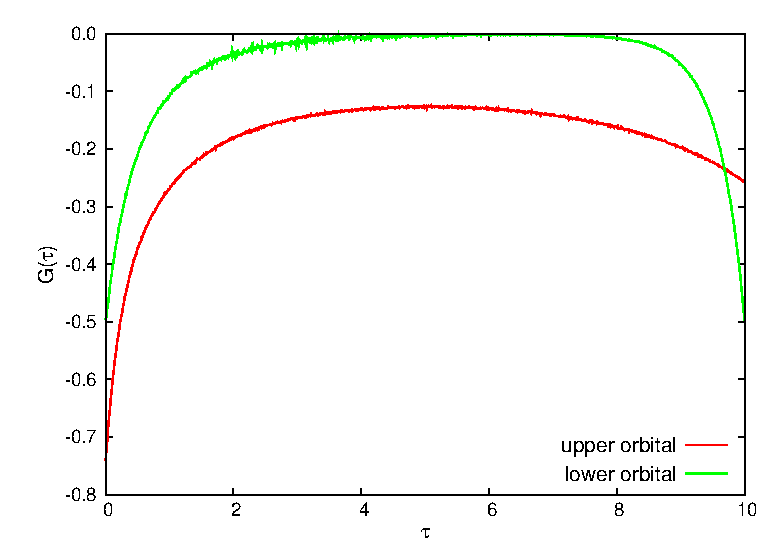
\includegraphics{figure/green-t823.eps}
\caption{包含晶体场劈裂的两带Hubbard模型的虚时格林函数$G(\tau)$} 
\label{fig:green-t823}
\end{figure}

\begin{figure}
\centering
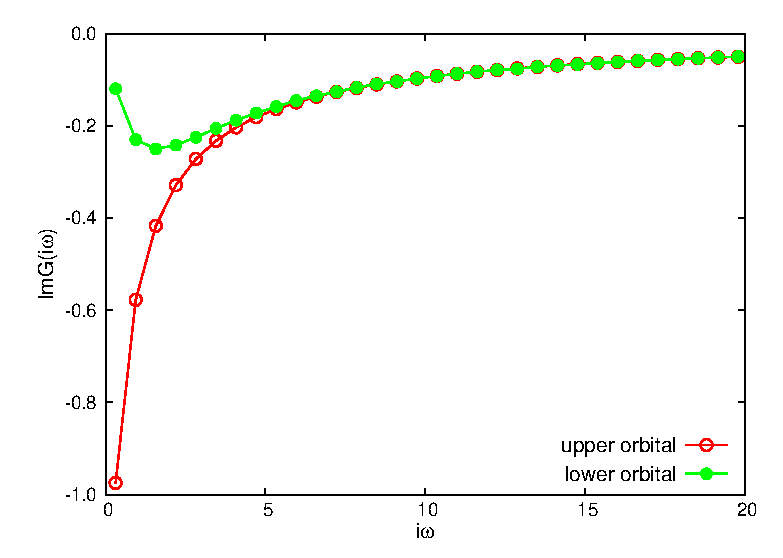
\includegraphics{figure/grn-t823.eps}
\caption{包含晶体场劈裂的两带Hubbard模型的虚频格林函数的虚部$\Im G(i\omega)$} 
\label{fig:grn-t823}
\end{figure}

确认计算完成后,用户可以按照第\ref{sec:basic}节中介绍的方法分析计算结果。在
这里分析任务就交给用户自己去完成了。我们计算结果如下: 图\ref{fig:green-t823}
展示的是虚时格林函数$G(\tau)$,图\ref{fig:grn-t823}展示的是虚频格林函数的虚
部$\Im G(i\omega)$。占据数情况如下:
\begin{itemize}
\item 能量高的轨道(upper orbital)的平均占据数为0.257216
\item 能量低的轨道(lower orbital)的平均占据数为0.500051
\end{itemize}

用户可以调整能带数目、相互作用强度、晶体场劈裂强度等参数,研究更为复杂的情况。
晶体场劈裂与Hund交换作用$J$相互耦合,可以诱发出具有轨道选择性的Mott金属$-$绝
缘体相变现象\footnote{相关的研究结果可以参阅{\color{red}arXiv:1203.5159}。}。

\subsection{动态屏蔽效应}
\label{subsec:scr}

此前我们所研究的Hubbard模型中,Coulomb相互作用强度$U$是一个恒定值,换言之
Coulomb相互作用是一个恒定的相互作用,但是实际情况并非如此。Coulomb相互
作用具有频率依赖性\footnote{此即所谓的动态屏蔽效应。},也就是说:
\begin{equation}
U = U(\omega)
\end{equation}
以金属Gd为例,当频率$\omega$由0变化至3\ eV时,$U(\omega)$由6.5\ eV
变化至17\ eV。再例如金属Ce,当频率由0变化至4\ eV时,$U(\omega)$由
3.5\ eV变化至7\ eV。我们定义$U_{0} = U(\omega = 0)$,在传统的LDA + $U$
计算或者是LDA + DMFT计算中,通常忽略掉Coulomb相互作用的频率依赖性,
而仅仅考虑$U_{0}$的效果。P. Werner在段表示算法的基础上发展了一套
全新的算法,可以将$U$的频率依赖性严格考虑进去\cite{werner:2010}。
我们在{\narcissus}组件中也实现了该算法,因此在本小节,我们将演示如
何使用{\narcissus}组件研究$U$随频率变化的单带半满Hubbard模型。

我们分别采用如下两种模型来描述$U$的频率依赖性:

plasmon pole模型
\begin{equation}
\label{eq:ppm}
\text{Re} U(\omega) = U + \frac{2\lambda^{2}\omega^{\prime}}{\omega^{2} - \omega^{\prime 2}}
\end{equation}

ohmic模型
\begin{equation}
\label{eq:om}
\text{Re} U(\omega) = U + \alpha \omega \ln \left|\frac{\omega_{c} + \omega}{\omega_{c} - \omega}\right| - 2\alpha \omega_{c}
\end{equation}

在{\narcissus}组件中,我们设计了isscr参数(请参阅第\ref{sec:isscr}节)
来控制是否激活动态屏蔽效应计算功能,并且通过lc参数(请参阅第\ref{sec:lc}
节)与wc参数(请参阅第\ref{sec:wc}节)来设定具体的plasmon pole模型或者是ohmic模
型。在本案例中,我们考虑如下的单带半满模型: $U = 6.0$\ eV,
$\lambda = \omega^{\prime} = \alpha = \omega_{c} = 1.0$,相应的plasmon pole
模型与ohmic模型如下图\ref{fig:scr-model}所示。

\begin{figure}
\centering
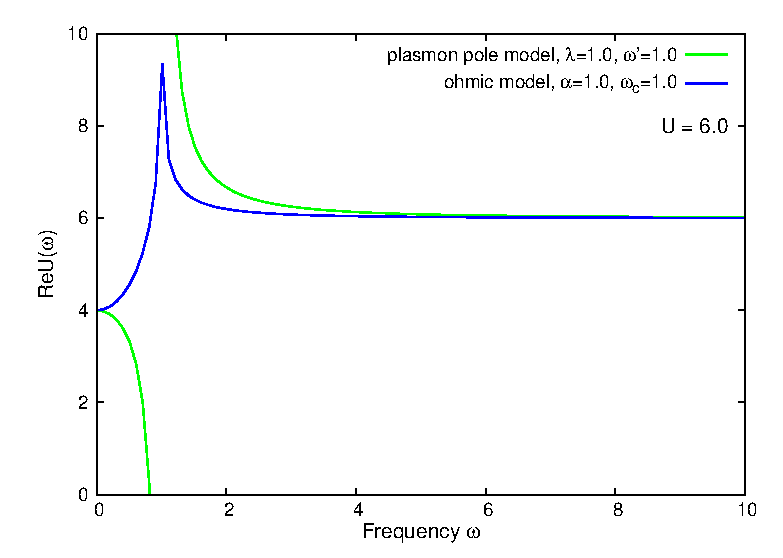
\includegraphics{figure/model.eps}
\caption{plasmon pole模型与ohmic模型示意图} 
\label{fig:scr-model}
\end{figure}

具体的计算流程如下所示。

步骤1:\underline{创建自己的工作目录/工作文件夹}

首先创建iqist\_test文件夹,该文件夹可作为用户的练习目录。如果用户在
练习上一个案例时已经创建了此文件夹,那么可以略过此操作。

在iqist\_test文件夹下创建子文件夹t824:

\noindent\colorbox{pink}{\parbox[r]{\linewidth}{\quad \$ mkdir t824 }}

再进入到t824文件夹中:

\noindent\colorbox{pink}{\parbox[r]{\linewidth}{\quad \$ cd t824 }}

那么当前所在的位置就是/iqist\_test/t824。

步骤2:\underline{准备solver.ctqmc.in}

在/opt/iqist/tutor/t824文件夹中,我们已经准备好了{\narcissus}组件的输入
文件solver.ctqmc.in,请将它复制到当前目录下,例如:

\noindent\colorbox{pink}{\parbox[r]{\linewidth}{\quad \$ cp /opt/iqist/tutor/t824/solver.ctqmc.in . }}

此solver.ctqmc.in文件的关键设置如下:
\begin{itemize}
  \item 采用自洽计算模式,isscf = 2
  \item 不计算任何高阶关联函数,isvrt = 1
  \item 不激活动态屏蔽效应计算,isscr = 1
  \item 该模型有1条能带,nband = 1
  \item 自旋投影方向,nspin = 2
  \item 轨道数目,norbs = 2
  \item 原子组态数目,ncfgs = 4
  \item 最大DMFT自洽迭代次数,niter = 20
  \item 库仑相互作用强度,$U$ = $U_{c}$ = $U_{v}$ = 6.0 
  \item Hund交换作用强度,$J_{z}$ = $J_{s}$ = $J_{p}$ = 0.0
  \item $U(\omega)$的模型参数,lc = wc = 0.0
  \item 化学势,mune = 3.0
  \item 反温度,beta = 10.0
  \item 最近邻跃迁系数,part = 0.50
\end{itemize}

在本案例中,我们分别计算以下三种情况:
\begin{itemize}
\item 静态Coulomb相互作用,$U = U_{0} = 6.0$\ eV
\item 动态屏蔽效应$U(\omega)$,plasmon pole模型,$\lambda = \omega^{\prime} = 1.0$
\item 动态屏蔽效应$U(\omega)$,ohmic模型,$\alpha = \omega_{c} = 1.0$
\end{itemize}
此处首先考虑第一种情况,因此将isscr设为1,而将lc与wc参数全部置为0.0。

步骤3:\underline{启动{\narcissus}组件进行实际计算}

在此案例中,我们使用8个计算核心运行{\narcissus}组件的ctqmc程序,用户可以根据现
有的计算资源做出适当调整。具体命令如下:

\noindent\colorbox{pink}{\parbox[r]{\linewidth}{\quad \$ nohup mpiexec -n 8 ctqmc < /dev/null >  out.dat \&}}

步骤4:\underline{监测{\narcissus}组件的运行状态}

请用户按照之前讲述的方法监测程序运行状态。

步骤5:\underline{plasmon pole模型计算}

当静态模型的计算完毕后,注意保存计算结果。然后使用vim编辑器打开solver.ctqmc.in
文件,将isscr参数的值修改为3,lc参数\footnote{亦即公式(\ref{eq:ppm})中的$\lambda$
参数。}的值修改为1.0,wc参数\footnote{亦即公式(\ref{eq:ppm})中的$\omega^{\prime}$
参数。}的值修改为1.0,然后保存退出。按照步骤3与步骤4的做法启动{\narcissus}组件
进行计算。此时,{\narcissus}组件将求解一个具有动态Coulomb相互作用的单带半满Hubbard
模型,而$U$的频率依赖性由plasmon pole模型近似描述。

步骤6:\underline{ohmic模型计算}

当plasmon pole模型的计算完毕后,注意保存计算结果。然后使用vim编辑器打开solver.ctqmc.in
文件,将isscr参数的值修改为4,lc参数\footnote{亦即公式(\ref{eq:om})中的$\alpha$
参数。}的值修改为1.0,wc参数\footnote{亦即公式(\ref{eq:om})中的$\omega^{c}$
参数。}的值修改为1.0,然后保存退出。按照步骤3与步骤4的做法启动{\narcissus}组件
进行计算。此时,{\narcissus}组件将求解一个具有动态Coulomb相互作用的单带半满Hubbard
模型,而$U$的频率依赖性由ohmic模型近似描述。

步骤7:\underline{数据的分析和处理}

\begin{figure}
\centering
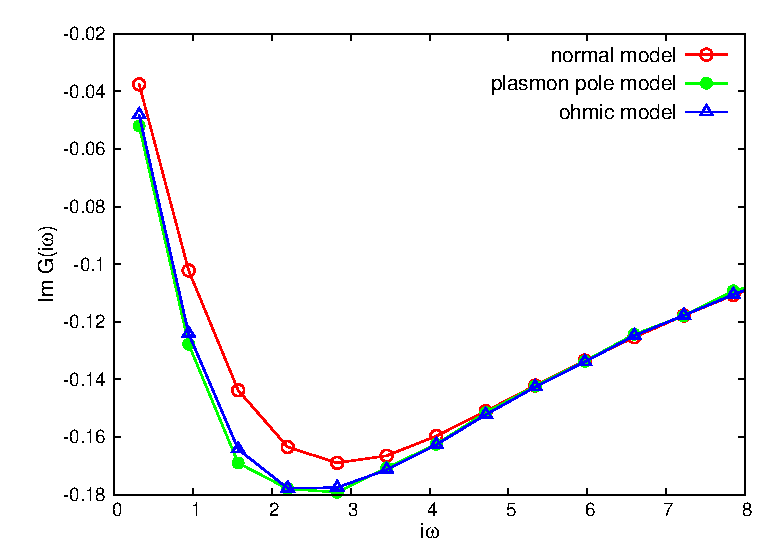
\includegraphics{figure/scr-grn.eps}
\caption{包含动态屏蔽效应的单带半满Hubbard模型的虚频格林函数的虚部$\Im G(i\omega)$} 
\label{fig:scr-grn}
\end{figure}

\begin{figure}
\centering
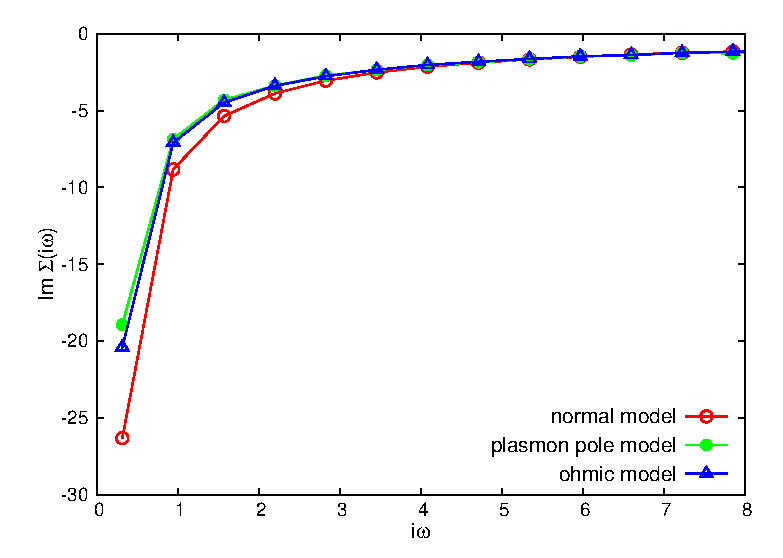
\includegraphics{figure/scr-sgm.eps}
\caption{包含动态屏蔽效应的单带半满Hubbard模型的电子自能函数的虚部$\Im \Sigma(i\omega)$} 
\label{fig:scr-sgm}
\end{figure}

在漫长的等待过后,计算终于成功结束了。在确认计算完成后,用户可以按照
第\ref{sec:basic}节中介绍的方法分析计算结果。在这里分析任务就交给用户
自己去完成了。我们计算结果如下:图\ref{fig:scr-grn}展示的是
虚频格林函数的虚部$\Im G(i\omega)$;图\ref{fig:scr-sgm}展示的是电子自能函数
的虚部$\Im \Sigma(i\omega)$。显而易见,动态屏蔽效应对$G(i\omega)$与$\Sigma(i\omega)$
均有十分重大的影响。

用户还可以变换isscr、$U_{c}$、$U_{v}$、lc与wc等参数的值,重复进行上
述计算,深入探讨动态屏蔽效应对于关联电子系统电子结构的影响。

\section{进阶应用II:物理量的精确测量}
\label{sec:stage2}

本节将介绍如何使用量子杂质求解器组件精确测定各种关键的物理量。

\subsection{单步执行模式}
\label{subsec:single}

在本小节里,我们简单的说明一下如何启用量子杂质求解器的单步执行模式。所谓的单步
执行模式,指的是量子杂质求解器不做DMFT迭代计算,仅仅只求解量子杂质模型一次。单
步执行模式主要有两种用途:

\begin{itemize}
\item 在LDA + DMFT计算模式中,量子杂质模型求解器必须以单步模式运行
\item 在自洽迭代已经完成后,精确测定特定的物理量
\end{itemize}

进入单步计算模式十分简单,用户只需要在solver.ctqmc.in输入文件里设置控制参数
isscf = 1即可(请参阅第\ref{sec:isscf}节)。如果用户希望用已经得到的杂化函
数\footnote{该杂化函数由量子杂质求解器组件生成。}作为输入,那么用户只需要
将包含杂化函数的数据文件solver.hyb.dat重命名为solver.hyb.in即可。特别注
意:如果用户使用的是其它程序产生的杂化函数,请预先转化为{\iqist}杂化函数
的特有格式(请参阅第\ref{sec:shi}节)。

\subsection{data binning模式}
\label{subsec:binning}

所谓的data binning模式,指的是在Monte Carlo抽样统计过程中,每间隔固定的时
间,将观测量打包输出。当程序结束后,我们将获得一个个数据包,这些数据包通
常称之为bin。那么bin的数目取决于抽样时间以及间隔时间的长短。我们在量子杂
质求解器组件中设计这么一种data binning模式,主要目的是精确测定虚时格林函
数$G(\tau)$或者是其它的物理量。在本小节中,我们将展示如何进入data binning
计算模式,为基于最大熵方法的解析延拓程序\footnote{亦即{\hibiscus}组件的entropy
程序,请参阅第\ref{sec:hib-ent}节。}积累虚时格林函数的抽样样本。解析
延拓程序将从这些样本数据中抽取出重要的统计信息,例如协方差。

data binning模式产生的data bin文件以solver.green.bin.*为名,其中*号代
表bin的编号。要进行data binning计算很简单,其实就是在做完DMFT自洽计算
之后,以最后收敛得到的虚频杂化函数$\Delta(i\omega)$为输入再做一次单步
计算。此前,我们已经在第\ref{subsec:1band}小节中自洽求解了一个单带半
满Hubbard模型,获得了收敛后的虚频杂化函数。现在我们将以此为基础来进
行data binning计算,我们的目标是要产生100个data bins。具体的计算流
程如下。

步骤1:\underline{创建自己的工作目录/工作文件夹}

首先创建iqist\_test文件夹,该文件夹可作为用户的练习目录。如果用户在练习
上一个案例时已经创建了此文件夹,那么可以略过此操作。

在iqist\_test文件夹下创建子文件夹t832:

\noindent\colorbox{pink}{\parbox[r]{\linewidth}{\quad \$ mkdir t832 }}

再进入到t832文件夹中:

\noindent\colorbox{pink}{\parbox[r]{\linewidth}{\quad \$ cd t832 }}

那么当前所在的位置就是/iqist\_test/t832。

步骤2:\underline{准备solver.ctqmc.in}

在/opt/iqist/tutor/t832文件夹中,我们已经准备好了{\azalea}组件的输入文
件solver.ctqmc.in,请将它复制到当前目录下,例如:

\noindent\colorbox{pink}{\parbox[r]{\linewidth}{\quad \$ cp /opt/iqist/tutor/t832/solver.ctqmc.in . }}

在solver.ctqmc.in文件中,有如下几个地方需要特别注意:

\begin{itemize}
  \item 设置单步计算模式,isscf = 1
  \item 设置data binning计算模式,isbin = 2
  \item nwrite = nsweep / 100,这样就能产生100个data bins
\end{itemize}

步骤3:\underline{准备solver.hyb.in}

除了solver.ctqmc.in文件以外,solver.hyb.in也是必须的输入文件,它提供了
初始化的杂化函数$\Delta(i\omega)$。
在/opt/iqist/tutor/t832文件夹中,我们已经准备好了{\azalea}组件的输入文
件solver.hyb.in,请将它复制到当前目录下,例如:

\noindent\colorbox{pink}{\parbox[r]{\linewidth}{\quad \$ cp /opt/iqist/tutor/t832/solver.hyb.in . }}

实际上,用户完全可以不使用我们所提供的solver.hyb.in文件。用户在完成例子t811
后(参阅第\ref{subsec:1band}小节),可以将最后得到杂化函数文件solver.hyb.dat
重命名为solver.hyb.in,然后将其拷贝到当前目录下即可,结果应该是完全一样的。

步骤4:\underline{启动{\azalea}组件进行实际计算}

在此案例中,我们使用8个计算核心运行{\azalea}组件的ctqmc程序,用户可以根据现
有的计算资源做出适当调整。具体命令如下:

\noindent\colorbox{pink}{\parbox[r]{\linewidth}{\quad \$ nohup mpiexec -n 8 ctqmc < /dev/null >  out.dat \&}}
此案例所须的运行时间较长,请用户耐心等待。

步骤5:\underline{数据的分析和处理}

计算结束后,用户就能得到100个data bins文件。在讲述后处理的章节时,我们将要用
这些数据来进行最大熵解析延拓(请参阅第\ref{subsec:ac-g}小节)。

最后需要提醒的一点是,如果用户希望获得更多的data bins,例如1000个,请不要简
单的将nsweep参数扩大100倍,因为这有可能导致integer类型的nsweep参数溢出。目
前最好的方法是建立10个imp\_bin*文件夹,分别进行上述计算。

\subsection{虚时格林函数}
\label{subsec:itime}

虚时格林函数$G(\tau)$是量子杂质求解器组件所输出的最重要的观测量之一。那么为了
获取精确的$G(\tau)$数据,用户可以遵循以下的规则。

\begin{itemize}
\item 采用并行模式运行量子杂质求解器(请参阅第\ref{sec:run_iqist}节)。{\iqist}
的量子杂质求解器组件对于计算核心的数目没有任何限制。一般而言,在其它条件相同
的情况下,计算核心的数目越多,所获得的计算结果就越精确。

\item 增加Monte Carlo抽样的次数(nsweep参数,请参阅第\ref{sec:nsweep}节)。在其它
条件相同的情况下,抽样次数越多,所获得的计算结果就越精确。

\item 适当减少抽样间隔(ncarlo参数,请参阅第\ref{sec:ncarlo}节)。在自关联程度
得到控制的前提下,减少抽样间隔就相当于增加抽样次数,有利于获得更精确的计算结果。

\item 采用data binning计算模式(isbin参数,请参阅第\ref{sec:isbin}节)。采用data
binning计算模式就相当于增加抽样次数十倍,有利于获得更精确的计算结果。

\item 采用正交多项式方法测量$G(\tau)$(isort参数,请参阅第\ref{sec:isort}
节)\footnote{注意:此方法不是对所有量子杂质求解器组件都适用。使用此方法还
需要仔细调整lemax参数(请参阅第\ref{sec:lemax}节)或者是chmax参数(请参阅
第\ref{sec:chmax}节),否则会弄巧成拙。}。
对于具有金属性质的系统而言,应用正交多项式方法能够获得十分平滑的虚时格林函数。
对于具有绝缘体性质的系统而言,正交多项式方法的计算结果不佳,但是可以采用内核
多项式方法对其进行矫正,详情请参阅附录\ref{app:kpm}。

\item 选择合适的虚时点数目(ntime参数,请参阅第\ref{sec:ntime}节)。一般而
言,ntime参数越大,抽样结果越精确,但是会大大降低计算效率,因此我们需要做
出折衷的选择。此外ntime的取值与beta参数也有密切的联系。

\item 适当进行强制对称化(isspn参数与issun参数,请参阅第\ref{sec:isspn}节与
第\ref{sec:issun}节)。如果系统的不同轨道之间存在着某种对称性,那么对它们进
行强制对称化有助于提高计算精度。

\end{itemize}

\subsection{虚频格林函数与电子自能函数}
\label{subsec:ifreq}

虚频格林函数$G(i\omega)$与电子自能函数$\Sigma(i\omega)$是十分重要的物理量,
应用{\iqist}软件包中的量子杂质求解器组件同样可以直接测量它们的值。那么如何
获得精确的测量值呢?请用户遵循下面的规则\footnote{下述规则与第\ref{subsec:itime}
小节中精确测量$G(\tau)$的规则基本雷同。}。

\begin{itemize}
\item 采用并行模式运行量子杂质求解器(请参阅第\ref{sec:run_iqist}节)。{\iqist}
的量子杂质求解器组件对于计算核心的数目没有任何限制。一般而言,在其它条件相同
的情况下,计算核心的数目越多,所获得的计算结果就越精确。

\item 增加Monte Carlo抽样的次数(nsweep参数,请参阅第\ref{sec:nsweep}节)。在其它
条件相同的情况下,抽样次数越多,所获得的计算结果就越精确。

\item 适当减少抽样间隔(nmonte参数,请参阅第\ref{sec:nmonte}节)。在自关联程度得
到控制的前提下,减少抽样间隔就相当于增加抽样次数,有利于获得更精确的计算结果。

\item 采用data binning计算模式(isbin参数,请参阅第\ref{sec:isbin}节)。采用data
binning计算模式就相当于增加抽样次数十倍,有利于获得更精确的计算结果。

\item 采用正交多项式方法测量$G(i\omega)$与$\Sigma(i\omega)$(isort参数,请参阅
第\ref{sec:isort}节)\footnote{注意:此方法不是对所有量子杂质求解器组件都适用,要
求isort参数取4 $\sim$ 6(仅{\gardenia}组件与{\narcissus}组件支持)。使用此方法还
需要仔细调整lemax参数(请参阅第\ref{sec:lemax}节)或者是chmax参数(请参阅
第\ref{sec:chmax}节),否则会弄巧成拙。}。对于具有金属性质的系统
而言,应用正交多项式方法能够获得十分平滑的结果。对于具有绝缘体性质的系统而言,正
交多项式方法的计算结果不佳,但是可以采用内核多项式方法对其进行矫正,详情请参阅附
录\ref{app:kpm}。

\item 选择合适的虚时点数目(ntime参数,请参阅第\ref{sec:ntime}节)。一般而
言,ntime参数越大,抽样结果越精确,但是会大大降低计算效率,因此我们需要
做出折衷的选择。此外ntime的取值与beta参数也有密切的联系。

\item 适当进行强制对称化(isspn参数与issun参数,请参阅第\ref{sec:isspn}节与
第\ref{sec:issun}节)。如果系统的不同轨道之间存在着某种对称性,那么对它们进
行强制对称化有助于提高计算精度。

\end{itemize}

\subsection{自旋$-$自旋关联函数与轨道$-$轨道关联函数}
\label{subsec:ssoo}

在本小节中,我们将展示如何使用{\gardenia}组件来计算自旋$-$自旋关联函数
以及轨道$-$轨道关联函数。从原理上说,在DMFT自洽计算过程中可以一并测量
这些关联函数,但是这样做无疑会加重计算负担,并且所获得的关联函数并不是
正确值。因此通常的做法是在DMFT自洽迭代计算完成后,进行一次单步计算(请
参阅第\ref{subsec:single}小节),专注于测量相关的物理量,这其中自然也包
括了关联函数。此前,我们已经在第\ref{subsec:1band}小节中自洽求解了一个
单带半满Hubbard模型,获得了收敛后的虚频杂化函数。那么现在我们将以此为
基础进行单步计算,精确测量自旋$-$自旋关联函数与轨道$-$关联函数。具体计
算流程如下。

步骤1:\underline{创建自己的工作目录/工作文件夹}

首先创建iqist\_test文件夹,该文件夹可作为用户的练习目录。如果用户在练习
上一个案例时已经创建了此文件夹,那么可以略过此操作。

在iqist\_test文件夹下创建子文件夹t835:

\noindent\colorbox{pink}{\parbox[r]{\linewidth}{\quad \$ mkdir t835 }}

再进入到t835文件夹中:

\noindent\colorbox{pink}{\parbox[r]{\linewidth}{\quad \$ cd t835 }}

那么当前所在的位置就是/iqist\_test/t835。

步骤2:\underline{准备solver.ctqmc.in}

在进行普通的DMFT自洽计算时,我们可以选用{\azalea}组件。但是由于{\azalea}组件不
具备计算自旋$-$自旋关联函数以及轨道$-$轨道关联函数的功能,我们必须弃用它而选用
具有此功能的{\gardenia}组件或者是{\narcissus}组件。

在/opt/iqist/tutor/t835文件夹中,我们已经准备好了{\gardenia}组件的输入文
件solver.ctqmc.in,请将它复制到当前目录下,例如:

\noindent\colorbox{pink}{\parbox[r]{\linewidth}{\quad \$ cp /opt/iqist/tutor/t835/solver.ctqmc.in . }}

在此solver.ctqmc.in文件中,有如下几个地方需要特别注意:
\begin{itemize}
  \item 设定单步计算模式,isscf = 1
  \item 无需采用data binning模式,isbin = 1
  \item 采用Legendre正交多项式方法测量虚时格林函数,isort = 2
  \item 计算自旋$-$自旋关联函数,isvrt = 2
  \item Legendre正交多项式的最大展开阶数,lemax = 24
  \item Legendre正交多项式线性网格点数目,legrd = 20001
  \item nffrq,nbfrq参数不起作用,可任意设置
\end{itemize}
其它的输入参数雷同于第\ref{subsec:1band}小节中的设置。

步骤3:\underline{准备solver.hyb.in}

除了solver.ctqmc.in文件以外,solver.hyb.in也是必须的输入文件,它提供了
初始化的杂化函数$\Delta(i\omega)$。
在/opt/iqist/tutor/t835文件夹中,我们已经准备好了{\gardenia}组件的输入文
件solver.hyb.in,请将它复制到当前目录下,例如:

\noindent\colorbox{pink}{\parbox[r]{\linewidth}{\quad \$ cp /opt/iqist/tutor/t835/solver.hyb.in . }}

实际上,用户完全可以不使用我们所提供的solver.hyb.in文件。用户在完成例子t811
后(参阅第\ref{subsec:1band}小节),可以将最后得到杂化函数文件solver.hyb.dat
重命名为solver.hyb.in,然后将其拷贝到当前目录下即可,结果应该是完全一样的。
虽然此solver.hyb.in文件是由{\azalea}组件输出的,但是{\gardenia}组件可以正确
读取它。

步骤4:\underline{启动{\gardenia}组件进行实际计算}

在此案例中,我们使用8个计算核心运行{\gardenia}组件的ctqmc程序,用户可以根据
现有的计算资源做出适当调整。具体命令如下:

\noindent\colorbox{pink}{\parbox[r]{\linewidth}{\quad \$ nohup mpiexec -n 8 ctqmc < /dev/null >  out.dat \&}}
该计算在大约两分钟之内就能完成。

步骤5:\underline{数据的分析和处理}

\begin{figure}
\centering
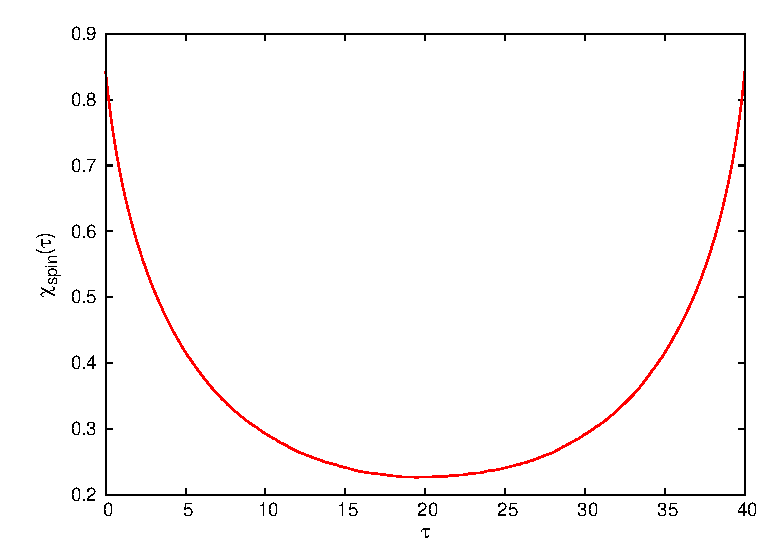
\includegraphics{figure/schi.eps}
\caption{单带半满Hubbard模型的自旋$-$自旋关联函数$\chi_{\text{spin}}(\tau)$} 
\label{fig:schi}
\end{figure}

计算完成后,首先还是要照例检查out.dat文件,确认该次计算有效。然后用gnuplot画图
比较该次计算得到的虚时格林函数和第\ref{subsec:1band}小节中计算得到的虚时格林函数。
它们应该非常吻合,否则就是出现错误了。

接下来我们用gnuplot画出自旋$-$自旋关联函数,该函数的数据存储在solver.schi.dat文
件中,如图\ref{fig:schi}所示,用户可以自行比较自己的计算结果。用户还可以利用
{\hibiscus}组件中的makechi程序对solver.schi.dat文件进行后处理,通过计算得到
有效局域磁矩$M_{e}$,详情请参阅第\ref{sec:hib-tool}节。

步骤6:\underline{轨道$-$轨道关联函数的计算}

\begin{figure}
\centering
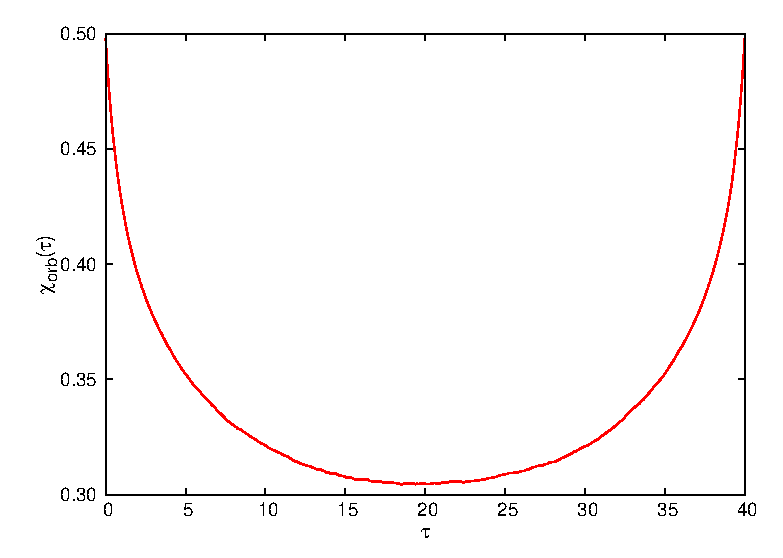
\includegraphics{figure/ochi.eps}
\caption{单带半满Hubbard模型的轨道$-$轨道关联函数$\chi_{\text{orb}}(\tau)$} 
\label{fig:ochi}
\end{figure}

在上述步骤中只是计算了自旋$-$自旋关联函数,我们也可以通过类似的步骤计算轨
道$-$轨道关联函数。请修改上述solver.ctqmc.in文件,将isvrt参数的取值设为3,
重新进行计算即可获得轨道$-$轨道关联函数。相关计算结果存储在solver.ochi.dat文
件中,我们可以用gnuplot软件对其进行绘图,结果如图\ref{fig:ochi}所示。

\subsection{双粒子格林函数与顶角函数}
\label{subsec:vertex}

在本小节中,我们将展示如何使用{\gardenia}组件来计算双粒子格林函
数$\chi(\omega,\omega^{\prime},\nu)$以及顶角函数
$\mathcal{F}(\omega,\omega^{\prime},\nu)$,这两种函数在DMFT理论
的非局域扩展中有着十分重要的应用\cite{slezak:435604,rubtsov:033101,toschi:045118}。
双粒子格林函数以及顶角函数的计算十分费时,我们通常是在DMFT自洽计
算结束后,再开启单步计算模式(请参阅第\ref{subsec:single}小节),对
它们进行详细的计算。此前,我们已经在第\ref{subsec:1band}小节中自洽求解了
一个单带半满Hubbard模型,获得了收敛后的虚频杂化函数。那么现在我们将以此为
基础进行单步计算,精确测量双粒子格林函数与顶角函数。具体计
算流程如下\footnote{此计算流程与第\ref{subsec:ssoo}小节中介绍的
自旋$-$自旋关联函数以及轨道$-$轨道关联函数的计算流程十分类似。}。

步骤1:\underline{创建自己的工作目录/工作文件夹}

首先创建iqist\_test文件夹,该文件夹可作为用户的练习目录。如果用户在练习
上一个案例时已经创建了此文件夹,那么可以略过此操作。

在iqist\_test文件夹下创建子文件夹t836:

\noindent\colorbox{pink}{\parbox[r]{\linewidth}{\quad \$ mkdir t836 }}

再进入到t836文件夹中:

\noindent\colorbox{pink}{\parbox[r]{\linewidth}{\quad \$ cd t836 }}

那么当前所在的位置就是/iqist\_test/t836。

步骤2:\underline{准备solver.ctqmc.in}

在进行普通的DMFT自洽计算时,我们可以选用{\azalea}组件。但是由于{\azalea}
组件不具备计算双粒子格林函数以及顶角函数的功能,我们必须弃用它而选用
具有此功能的{\gardenia}组件或者是{\narcissus}组件。在本案例中,我们选用
的是{\gardenia}组件,如果需要考虑动态屏蔽效应对于双粒子格林函数以及顶角
函数的影响,那么必须使用{\narcissus}组件。

在/opt/iqist/tutor/t836文件夹中,我们已经准备好了{\gardenia}组件的输入文
件solver.ctqmc.in,请将它复制到当前目录下,例如:

\noindent\colorbox{pink}{\parbox[r]{\linewidth}{\quad \$ cp /opt/iqist/tutor/t836/solver.ctqmc.in . }}

在此solver.ctqmc.in文件中,有如下几个地方需要特别注意:
\begin{itemize}
  \item 设定单步计算模式,isscf = 1
  \item 无需采用data binning模式,isbin = 1
  \item 采用Legendre正交多项式方法测量虚时格林函数,isort = 2
  \item 计算双粒子格林函数以及顶角函数,isvrt = 4
  \item Legendre正交多项式的最大展开阶数,lemax = 24
  \item Legendre正交多项式线性网格点数目,legrd = 20001
  \item 设置费米频率点的数目,nffrq = 32
  \item 设置玻色频率点的数目,nbfrq = 2
\end{itemize}

其中,isvrt参数可以设置为4,也可以设置为5,这两种设置都能够得到双粒子格林
函数以及顶角函数。只不过前者的输出数据存储在solver.twop.dat文件中,而后者
的输出数据存储在solver.vrtx.dat文件中。后者所用的算法更为精确,计算量也更
大。关于isvrt参数的详情,请参阅第\ref{sec:isvrt}节。此外,利用正交多项式
方法可以有效地提升双粒子格林函数以及顶角函数的测量精度,因此在本案例中,
我们激活了Legendre正交多项式方法(isort参数,请参阅第\ref{sec:isort}节)。
为了提升计算效率,减少计算时间,费米频率点的数目(nffrq参数,请参阅
第\ref{sec:nffrq}节)以及玻色频率点的数目(nbfrq参数,请参阅第\ref{sec:nbfrq}
节)都设得比较小。如果要获得更精确的结果,请用户酌情增加这两个参数的值。
其它的输入参数雷同于第\ref{subsec:ssoo}小节中的设置。

步骤3:\underline{准备solver.hyb.in}

除了solver.ctqmc.in文件以外,solver.hyb.in也是必须的输入文件,它提供了
初始化的杂化函数$\Delta(i\omega)$。
在/opt/iqist/tutor/t836文件夹中,我们已经准备好了{\gardenia}组件的输入文
件solver.hyb.in,请将它复制到当前目录下,例如:

\noindent\colorbox{pink}{\parbox[r]{\linewidth}{\quad \$ cp /opt/iqist/tutor/t836/solver.hyb.in . }}

实际上,用户完全可以不使用我们所提供的solver.hyb.in文件。用户在完成例子t811
后(参阅第\ref{subsec:1band}小节),可以将最后得到杂化函数文件solver.hyb.dat
重命名为solver.hyb.in,然后将其拷贝到当前目录下即可,结果应该是完全一样的。
虽然此solver.hyb.in文件是由{\azalea}组件输出的,但是{\gardenia}组件可以正确
读取它。

步骤4:\underline{启动{\gardenia}组件进行实际计算}

在此案例中,我们使用8个计算核心运行{\gardenia}组件的ctqmc程序,用户可以根据
现有的计算资源做出适当调整。具体命令如下:

\noindent\colorbox{pink}{\parbox[r]{\linewidth}{\quad \$ nohup mpiexec -n 8 ctqmc < /dev/null >  out.dat \&}}

由于nffrq参数以及nbfrq参数取得比较小,计算量不大,该计算在大约两分钟之内就能
够完成。

步骤5:\underline{数据的分析和处理}

\begin{figure}
\centering
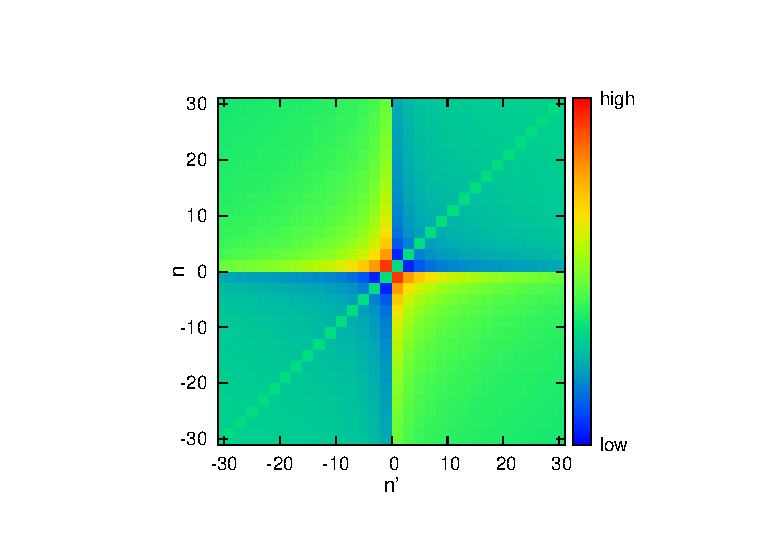
\includegraphics[scale=1.05]{figure/v_t.eps}
\caption[总的双粒子格林函数$\chi^{mn}_{\text{tot}}(\omega,\omega^{\prime},\nu)$]
{单带半满Hubbard模型的总的双粒子格林函数$\chi^{mn}_{\text{tot}}(\omega,\omega^{\prime},\nu)$。high = 120, low = -60。} 
\label{fig:v_t}
\end{figure}

\begin{figure}
\centering
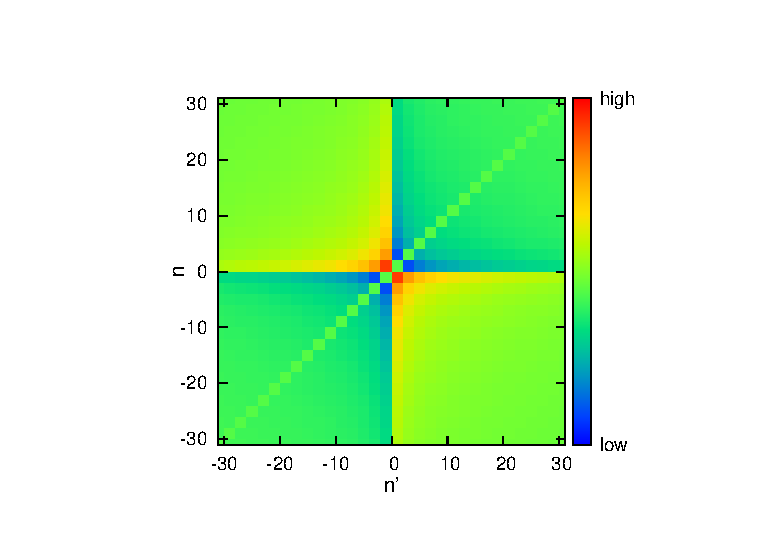
\includegraphics[scale=1.05]{figure/v_0.eps}
\caption[可约双粒子格林函数$\chi^{mn}_{0}(\omega,\omega^{\prime},\nu)$]
{单带半满Hubbard模型的可约双粒子格林函数$\chi^{mn}_{0}(\omega,\omega^{\prime},\nu)$。high = 100, low = -80。} 
\label{fig:v_0}
\end{figure}

\begin{figure}
\centering
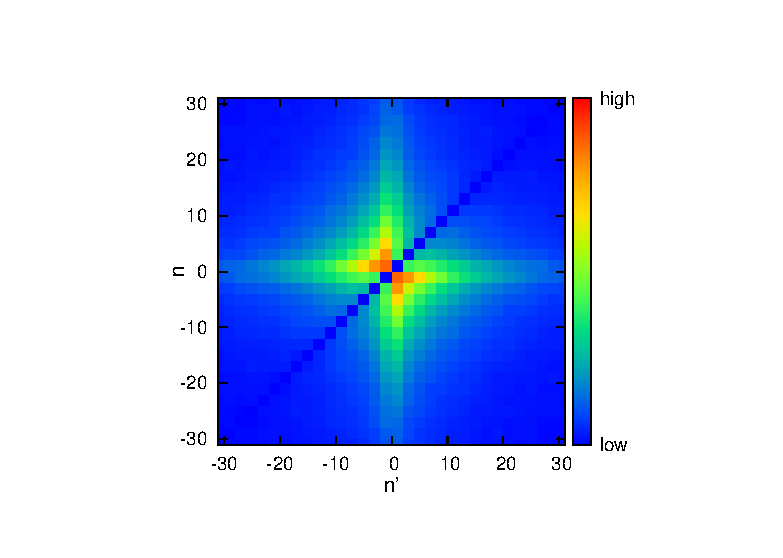
\includegraphics[scale=1.05]{figure/v_i.eps}
\caption[不可约双粒子格林函数$\chi^{mn}_{\text{irr}}(\omega,\omega^{\prime},\nu)$]
{单带半满Hubbard模型的不可约双粒子格林函数$\chi^{mn}_{\text{irr}}(\omega,\omega^{\prime},\nu)$。high = 25, low = 0。} 
\label{fig:v_i}
\end{figure}

\begin{figure}
\centering
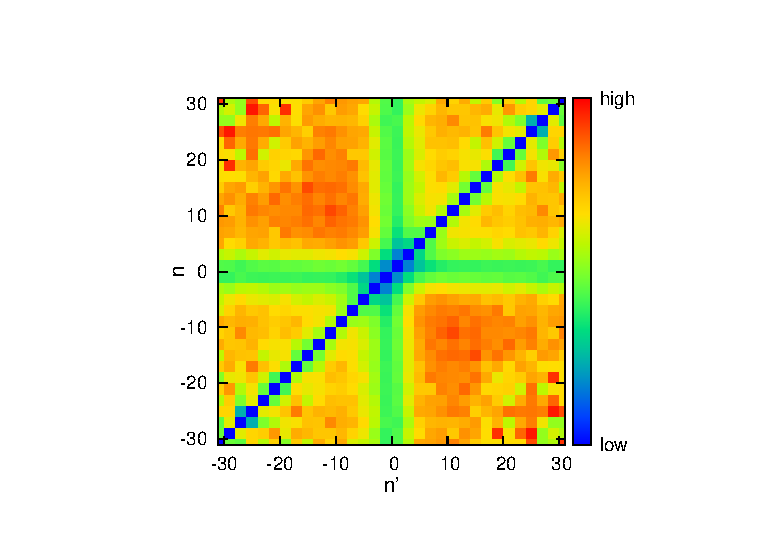
\includegraphics[scale=1.05]{figure/v_g.eps}
\caption[全顶角函数$\mathcal{F}^{mn}(\omega,\omega^{\prime},\nu)$]
{单带半满Hubbard模型的全顶角函数$\mathcal{F}^{mn}(\omega,\omega^{\prime},\nu)$。high = 25, low = 0。} 
\label{fig:v_g}
\end{figure}

计算完成后,首先还是要照例检查out.dat文件,确认该次计算有效。然后用gnuplot画图
比较该次计算得到的虚时格林函数和第\ref{subsec:1band}小节中计算得到的虚时格林函
数(请参阅图\ref{fig:green})。它们应该非常吻合,否则就是出现错误了。

接下来我们关注双粒子格林函数以及顶角函数的计算结果。由于isvrt参数设置为4,那么
相应的输出文件为solver.twop.dat。如果isvrt参数设置为5,那么输出文件为solver.vrtx.dat。
这两个文件的数据格式是完全一样的,详情请参阅第\ref{sec:file}节。在solver.twop.dat
(solver.vrtx.dat)文件中,有很多数据block,每个玻色频率点对应一个block。在本案例
中,由于nbfrq = 2,因此文件中一共有2个block。在绘图时,我们首先需要将block分离,
然后对每一个block单独绘图。下面的图\ref{fig:v_t}-图\ref{fig:v_g}分别绘制了
总的双粒子格林函数$\chi^{mn}_{\text{tot}}(\omega,\omega^{\prime},\nu)$、
可约双粒子格林函数$\chi^{mn}_{0}(\omega,\omega^{\prime},\nu)$、
不可约双粒子格林函数$\chi^{mn}_{\text{irr}}(\omega,\omega^{\prime},\nu)$以及
全顶角函数$\mathcal{F}^{mn}(\omega,\omega^{\prime},\nu)$。其中$\nu = 0$,亦即
图中的数据为第一个block中的数据。用户可以自行绘图,以检验计算结果是否准确。

最后,用户可以将isvrt参数设为5,重新进行上述计算,并比较前后两次的计算结果,
判明孰优孰劣。此外,用户还可以增加nffrq、nbfrq等参数的值,看看计算结果是否
有明显的改变。特别值得一提的是,isort参数的取值对于相关计算的精度有十分显
著的影响,这一切就留待用户去自行摸索了,此处不再赘述。

\section{进阶应用III:后处理步骤}
\label{sec:stage3}

本节专注于后处理步骤,介绍如何使用{\hibiscus}组件对$G(\tau)$和$\Sigma(i\omega)$
进行解析延拓,分别获取电子谱函数$A(\omega)$和实频电子自能$\Sigma(\omega)$。

\subsection{虚时格林函数的解析延拓}
\label{subsec:ac-g}

在本小节中,我们将演示在第\ref{subsec:binning}小节的基础上,如何使用
{\hibiscus}/hibiscus-entropy组件对虚时格林函数$G(\tau)$进行解析延
拓,得到谱函数$A(\omega)$。

步骤1:\underline{创建自己的工作目录/工作文件夹}

首先创建iqist\_test文件夹,该文件夹可作为用户的练习目录。如果用户在练习上一个案例
时已经创建了此文件夹,那么可以略过此操作。

在iqist\_test文件夹下创建子文件夹t841:

\noindent\colorbox{pink}{\parbox[r]{\linewidth}{\quad \$ mkdir t841 }}

步骤2:\underline{准备tau.grn.dat}

hibiscus-entropy组件需要的数据输入文件为tau.grn.dat,该文件包含了处理过
的$G(\tau)$数据。我们首先使用{\hibiscus}/hibiscus-toolbox组件下的maketau
程序产生tau.grn.dat文件。请进入在第\ref{subsec:binning}小节中所建立的
t832文件夹:

\noindent\colorbox{pink}{\parbox[r]{\linewidth}{\quad \$ cd t832 }}

请判明在t832目录下是否存在着100个data bins(亦即100个solver.green.bin.*
文件),如果答案是否定的,那么请按照第\ref{subsec:binning}小节中的介绍
首先执行例子t832;如果答案是肯定的,那么可以调用maketau程序进行处理。
maketau程序的可执行文件为mtau.x(详情请参阅第\ref{sec:hib-tool}节),运
行mtau.x的命令如下:

\noindent\colorbox{pink}{\parbox[r]{\linewidth}{\quad \$ mtau.x }}

用户只要根据程序提示一步一步输入控制参数就可以了。下面是一个运行例子:
\begin{lstlisting}[frame=single]
  MTAU
  making tau-dependent imaginary time green's function
  version: 2011.08.18T
 
  >>> number of bands (default = 1):
  >>> 1
 
  >>> number of time slice (default = 129 or 1024):
  >>> 1024
 
  >>> number of data bins (default = 1):
  >>> 100
 
  >>> file type generated by quantum impurity solver (default = 1):
  ctqmc: 1
  hfqmc: 2
  ctqmc: 3 (bin mode)
  hfqmc: 4 (bin mode)
  >>> 3
 
  >>> inversion of temperature (default = 10.0):
  >>> 40
 
  >>> reading solver.green.bin ...   1
  >>> status: OK
 
  >>> reading solver.green.bin ...   2
  >>> status: OK

  ....................................
\end{lstlisting}
对于maketau程序的主要控制参数,我们简单介绍如下:
\begin{itemize}
  \item 第6行,总的能带数,本例中只有1个能带。
  \item 第9行,总的虚时片数,本例中为1024
  \item 第12行,solver.green.bin*文件数目,本例中为100
  \item 第19行,杂质求解器类型,本例中为3
  \item 第22行,反温度$\beta$,本例中为40
\end{itemize}
当maketau程序运行完毕后,如果一切正常,那么即可获得
tau.grn.dat文件。请不要手动修改tau.grn.dat文件,而是把它
直接拷贝到t841文件夹:

\noindent\colorbox{pink}{\parbox[r]{\linewidth}{\quad \$ cp tau.grn.dat ../t841 }}

然后,我们进入到t841文件夹:

\noindent\colorbox{pink}{\parbox[r]{\linewidth}{\quad \$ cd ../t841 }}

那么当前所在目录就是t841。

步骤3:\underline{准备entropy.in}

hibiscus-entropy组件所需要的控制文件为entropy.in。如果没有entropy.in,
那么hibiscus-entropy组件将无法正常运行。在/opt/iqist/tutor/t841文件夹
中,我们已经准备好了hibiscus-entropy组件的输入文件entropy.in, 请将它复
制到当前目录下,例如:

\noindent\colorbox{pink}{\parbox[r]{\linewidth}{\quad \$ cp /opt/iqist/tutor/t841/entropy.in . }}

关于该输入文件的内容,请用户参考第\ref{sec:hib-ent}节中关于该文件的详
细介绍,此处不再赘述。

步骤4:\underline{启动hibiscus-entropy组件进行实际计算}

hibiscus-entropy组件的可执行程序名为entropy,这是一个串行程序,不支持
MPI并行,那么执行它的具体命令如下:

\noindent\colorbox{pink}{\parbox[r]{\linewidth}{\quad \$ nohup entropy </dev/null> out.dat \& }}
程序很快运行完毕,耗时约1分钟。

步骤5:\underline{数据分析和处理}

\begin{figure}
\centering
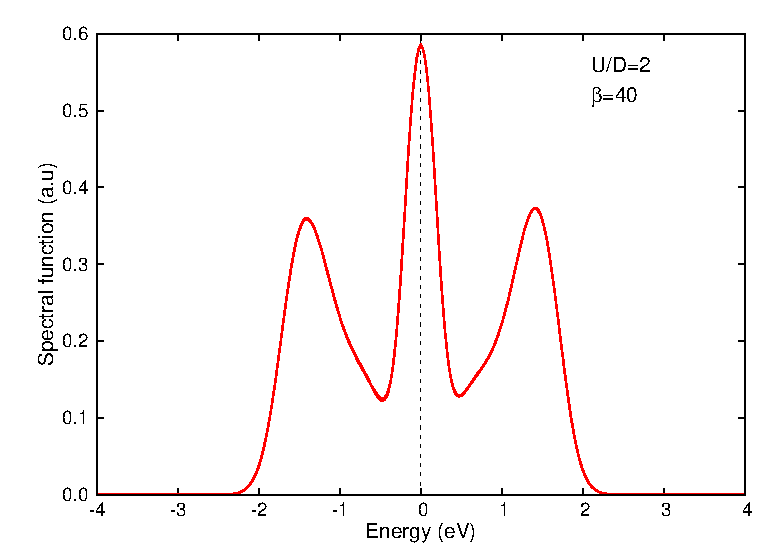
\includegraphics{figure/spec-t841.eps}
\caption{单带半满Hubbard模型的谱函数$A(\omega)$} 
\label{fig:spec-t841}
\end{figure}

entropy程序运行完毕后,所产生的谱函数$A(\omega)$储存于mem.dos.dat文件
中,用户可以使用gnuplot软件画出谱函数:

\noindent\colorbox{pink}{\parbox[r]{\linewidth}{\quad \$ gnuplot> plot "mem.dos.dat" u 1:2 w lp }}

具体结果如图\ref{fig:spec-t841}所示。在本案例中,Coulomb相互作用强度
还比较小,因而谱函数显示出典型的三峰结构。上下Hubbard带十分对称,这意味
着系统具有粒子$-$空穴对称性,处于半填满状态。

hibiscus-entropy组件基于最大熵方法\cite{jarrell:133},在{\iqist}软件包
中,我们还提供基于随机解析延拓方法\cite{beach}的hibiscus-stochastic组件。
利用hibiscus-stochastic组件也可以对$G(\tau)$进行解析延拓,得到电子谱函
数$A(\omega)$(详情请参阅第\ref{sec:hib-sai}节),用户不妨自行一试。

\subsection{虚频电子自能函数的解析延拓}
\label{subsec:ac-s}

在本小节中,我们将演示在第\ref{subsec:1band}小节的基础上,如何使用
{\hibiscus}/hibiscus-swing组件对虚频电子自能函数$\Sigma(i\omega)$
进行解析延拓,得到实频率上的自能信息$\Sigma(\omega)$。$\Sigma(\omega)$
对于LDA + DMFT计算而言十分有用,利用它可以进一步计算$A(k,\omega)$、光
电导等物理量。

为了获得{\hibiscus}/hibiscus-swing组件所需要的数据输入文件std.sgm.dat,我们首先
需要得到虚频自能函数的多个样本,然后再利用{\hibiscus}/hibiscus-toolbox
组件里的makestd程序处理这些样本,求得平均值和方差值等信息,生成std.sgm.dat
文件,最后才用{\hibiscus}/hibiscus-swing组件对其进行处理,获得最终的实频电子自能。下
面是详细的计算流程。

步骤1:\underline{创建自己的工作目录/工作文件夹}

首先创建iqist\_test文件夹,该文件夹可作为用户的练习目录。如果用户在练习上一个案例
时已经创建了此文件夹,那么可以略过此操作。

在iqist\_test文件夹下创建子文件夹t842:

\noindent\colorbox{pink}{\parbox[r]{\linewidth}{\quad \$ mkdir t842 }}

进入到t842文件夹中:

\noindent\colorbox{pink}{\parbox[r]{\linewidth}{\quad \$ cd t842 }}

那么当前所在的目录就是t842。在该文件夹中建立子文件夹sigm1,然后拷贝我们
预先准备好的输入文件solver.ctqmc.in到sigm1中:
 
\noindent\colorbox{pink}{\parbox[r]{\linewidth}{\quad \$ cp /opt/iqist/tutor/t842/solver.ctqmc.in  sigm1/ }}

然后拷贝t811文件夹中的solver.hyb.dat文件到sigm1文件夹中,并将其重命名为
solver.hyb.in:

\noindent\colorbox{pink}{\parbox[r]{\linewidth}{\quad \$ cp ../t811/solver.hyb.dat  sigm1/solver.hyb.in }}

如果在t811文件夹中不存在solver.hyb.dat文件,这说明用户还没有完成t811这个
案例。请用户按照第\ref{subsec:1band}小节中的指示,一步一步完成案例t811,
产生正确的solver.hyb.dat文件,再执行上述拷贝/重命名操作。

接下来请产生sigm1文件夹的9个拷贝,命名为sigm*,*从2变化到10,例如:

\noindent\colorbox{pink}{\parbox[r]{\linewidth}{\quad \$ cp -r sigm1  sigm2 }}

在t842文件夹下建立文件夹sigm\_std,用作预处理程序makestd的工作目录:

\noindent\colorbox{pink}{\parbox[r]{\linewidth}{\quad \$ mkdir sigm\_std }}

在t842文件夹下建立文件夹sigm\_swing,作为{\hibiscus}/hibiscus-swing组件的工作目录:

\noindent\colorbox{pink}{\parbox[r]{\linewidth}{\quad \$ mkdir sigm\_swing }}

步骤2:\underline{启动\azalea 组件进行计算}

依次进入每个sigm*目录,启动\azalea 组件进行计算,例如:

\noindent\colorbox{pink}{\parbox[r]{\linewidth}{\quad \$ nohup mpiexec -n 8 ctqmc < /dev/null > out.dat \& }}

实际上,此刻我们所做的即是第\ref{subsec:single}小节里所讲的单步计算模式。
由于{\azalea}组件的高效率,10次计算很快就能执行完毕。

步骤3:\underline{使用makestd程序对自能函数进行预处理}

分别将sigm*文件夹中的solver.sgm.dat文件依次拷贝到sigm\_std文件夹,并将其
重命名为solver.sgm.dat.*文件,例如:

\noindent\colorbox{pink}{\parbox[r]{\linewidth}{\quad \$ cp sigm1/solver.sgm.dat  sigm\_std/solver.sgm.dat.1 }}

然后进入到sigm\_std文件夹中,启动makestd程序进行自能预处理。makestd程序
的可执行程序名为mstd.x,执行命令如下:

\noindent\colorbox{pink}{\parbox[r]{\linewidth}{\quad \$ mstd.x }}

用户只需根据程序提示输入控制参数就可以了,具体如下所示:
\begin{lstlisting}[frame=single]
  MSTD
  making average and standard deviation for self-energy function
  version: 2011.08.18T
 
  >>> number of bands (default = 1):
  >>> 1
 
  >>> number of matsubara frequency points (default = 8193):
  >>> 8193
 
  >>> number of data bins (default = 1):
  >>> 10
 
  >>> reading solver.sgm.dat ...   1
  >>> status: OK
 
  >>> reading solver.sgm.dat ...   2
  >>> status: OK

  ....................................

\end{lstlisting}
对于makestd程序的主要控制参数,我们简单介绍如下:
\begin{itemize}
  \item 第6行,总的能带数,本例中只有1个能带
  \item 第9行,虚频率点数,本例中为8193
  \item 第12行,solver.sgm.dat.*文件数目,本例中为10
\end{itemize}
当makestd程序运行完毕后,如果一切正常,那么即可获得
std.sgm.dat文件。请不要手动修改std.sgm.dat文件,而是把它
直接拷贝到sigm\_swing文件夹中:

\noindent\colorbox{pink}{\parbox[r]{\linewidth}{\quad \$ cp std.sgm.dat  ../sigm\_swing }}

步骤4:\underline{使用hibiscus-swing组件进行自能解析延拓}

进入sigm\_swing文件夹,将我们预先准备好的metal.sh脚本文件拷贝到当前目录:

\noindent\colorbox{pink}{\parbox[r]{\linewidth}{\quad \$ cp /opt/iqist/tutor/t842/metal.sh  . }}

该文件是{\hibiscus}/hibiscus-swing组件的启动脚本。由于在本例中,该体系明显
处于金属相,因此我们使用metal.sh脚本来启动hibiscus-swing组件,反之
则应该使用insulator.sh脚本。对于该脚本,我们需要注意以下几点:
\begin{itemize}
  \item 请用户调整exec变量,指向hibiscus-swing组件所在目录。
  \item para变量中设置的参数请保持不变。
\end{itemize}
更多的关于hibiscus-swing组件的信息,请参考第\ref{sec:hib-swing}节中的介绍,
此处不再赘述。

下面请运行脚本metal.sh进行解析延拓操作,命令示例如下:

\noindent\colorbox{pink}{\parbox[r]{\linewidth}{\quad \$ ./metal.sh }}
该程序很快就会运行完毕,并且输出很多数据文件。

步骤5:\underline{数据分析和处理}

\begin{figure}
\centering
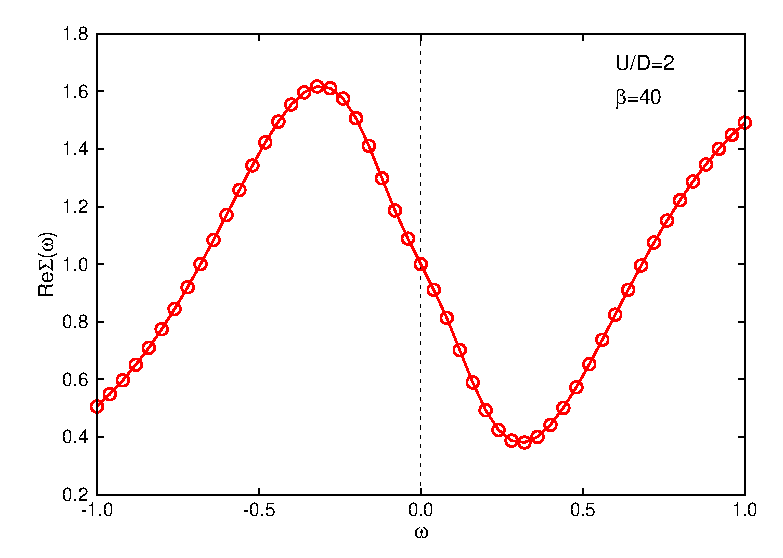
\includegraphics{figure/sigr-real.eps}
\caption{单带半满Hubbard模型实频电子自能的实部$\Re \Sigma (\omega)$} 
\label{fig:sigr-real}
\end{figure}

\begin{figure}
\centering
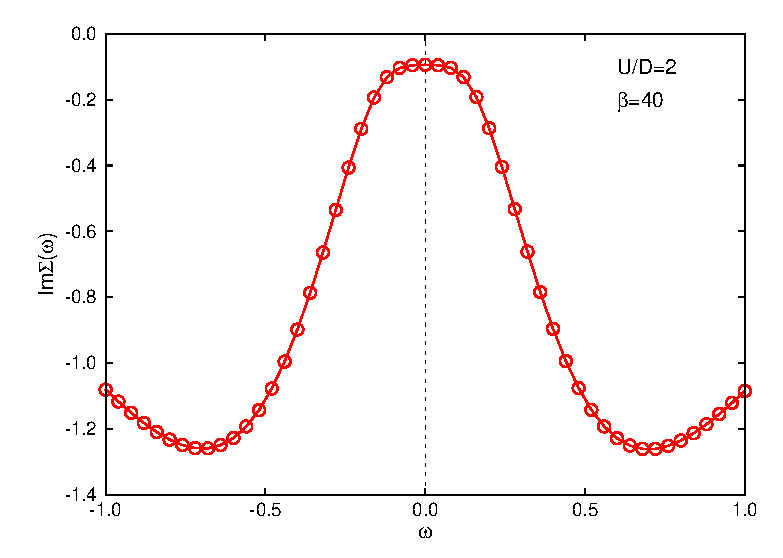
\includegraphics{figure/sigr-img.eps}
\caption{单带半满Hubbard模型实频电子自能的虚部$\Im \Sigma (\omega)$} 
\label{fig:sigr-img}
\end{figure}

{\hibiscus}/hibiscus-swing组件在运行过程中将会产生许多输出文件,具体信息请
参考第\ref{sec:hib-swing}节中的介绍。此刻我们只须关注sigr\_linear.out文件,
使用gnuplot软件画出实频电子自能的实部:

\noindent\colorbox{pink}{\parbox[r]{\linewidth}{\quad \$ gnuplot> plot [-1:1] "sigr\_linear.out" u 2:3 w lp }}

如图\ref{fig:sigr-real}所示,实频自能的实部在费米能级附近具有很好的线性行为,
这表示该系统具有很好的费米液体行为。该系统的谱函数即是第\ref{subsec:ac-g}小
节中所展示的图\ref{fig:spec-t841},结合谱函数更能明显看出该系统符合费米液体
理论的描述。

再使用gnuplot软件画出实频电子自能的虚部:

\noindent\colorbox{pink}{\parbox[r]{\linewidth}{\quad \$ gnuplot> plot [-1:1] "sigr\_linear.out" u 2:4 w lp }}

如图\ref{fig:sigr-img}所示,实频自能的虚部在费米能级附近趋于0,这也是费
米液体金属的典型行为。

\section{{\iqist}实战应用}
\label{sec:project}

在前面的章节中我们已经详细讲述了{\iqist}软件包里各个组件的使用方法,如果
用户是按照教程一步步操作下来的话,那么相信用户已经熟练掌握了{\iqist}软件
包的各种应用技能。本章的前几节展示的都是相对比较简单的案例,那么在这一节
中,我们将列举两个{\iqist}软件包实战应用的综合案例。第一个例子是两带
Hubbard模型中掺杂和晶体场劈裂相互作用导致的具有轨道选择性的Mott相变,
第二个例子是三带Anderson杂质模型中的轨道Kondo效应和自旋Kondo效应。在本节
中,我们首先简单叙述物理模型和计算细节,然后展示计算结果。至于详细的计算
过程和数据分析、作图等步骤,请用户独立完成,以此来检验用户是否熟练掌握了
前面教程的内容。下面我们就开始{\iqist}软件包的实战应用。

\subsection{两带Hubbard模型中掺杂与晶体场相互作用导致的轨道选择性Mott相变}

为了解释Ca$_{2-x}$Sr$_x$RuO$_4$材料中导带电子的混合性质,人们提出了所谓的
轨道选择性Mott相变的概念\cite{anisimov:191}。在该材料中,一部分导带电子表
现出巡游性质(具有金属性的电导),而另外一部分导带电子表现出局域性质(具有居
里$-$外斯特性的磁化系数)。经过长期的研究,人们提出了许多导致轨道选择性Mott
相变的机制\cite{koga:216402,koga:045128,medici:205124,ferrero:205126,
held:201102(R),knecht:081103(R),liebsch:226401,koga:359361,inaba:2393,
medici:126401,kita:195130,inaba:094712,jakobi:115109,werner:126405},请用
户参阅相关文献。

在本小节中,我们将研究在两带Hubbard模型中,在晶体场劈裂存在的情况下,由于
掺杂所导致的轨道选择性Mott相变。我们将主要计算该系统随着晶体场劈裂和电子
掺杂变化的相图。在初始的时候,该系统总的平均电子占据数为1,通过调节Coulomb
相互作用的强度使其处于金属$-$绝缘体相变的临界区域,但是依然处在金属相区域。
然后,我们对该系统进行电子掺杂,并且调节晶体场劈裂的大小,我们发现当电子掺
杂大于一定量之后,在一定晶体场范围内,系统进入了具有轨道选择性的Mott相(OSMP)
区域,即能级较低的那个轨道(半满)从金属相变为Mott绝缘相,而能级较高的那个轨
道依然保持为金属相。通过分析轨道占据数和局域磁矩,我们得出这样的结论:在Hund
交换作用存在的情况下,掺杂电子促使系统形成较大的局域磁矩,而局域磁矩的存在
会散射电子,从而导致有效的电子相互作用强度增加,促使能级较低的那个半满轨道
发生了从金属到Mott绝缘体的相变。

1.\underline{模型哈密顿量}

我们研究的两带Hubbard模型的哈密顿量如下:
\begin{equation}
\label{eqn:model}
\begin{split}
H = &-t\sum_{<i,j>,a\sigma} d_{i a \sigma}^{\dagger} d_{j a \sigma} 
     +\sum_{i, a \sigma} (-\mu + \Delta_{a})n_{a \sigma} \\
    &+U\sum_{i,a} n_{a \uparrow} n_{a \downarrow} 
     +\sum_{i,a>b,\sigma \sigma^{\prime}}(U^\prime-\delta_{\sigma\sigma^\prime}J) 
      n_{a \sigma}n_{b \sigma^\prime}
\end{split}
\end{equation}
其中,$d^{\dagger}$($d$)为$d$电子产生(消灭)算符,$a,b$为能带指标
($a,b = 1 \sim 2$),$\sigma,\sigma^{\prime}$为自旋指标,$n_{a \sigma} = 
d^{\dagger}_{a \sigma}d_{a \sigma}$为占据数算符,$\mu$为化学势,
$\Delta$为杂质能级。$U$($U'$)分别为轨道间(轨道内)Coulomb相互作用,
$J$为Hund交换相互作用,我们采取如下限制$U=U^{\prime}+2J$。

2.\underline{计算细节}

由于上述哈密顿量具有密度$-$密度相互作用的形式(不包括自旋翻转和对跃迁项,请
参阅公式(\ref{eq:loc})),我们将使用{\iqist}软件包的{\azalea}组件计算其相图。
我们还会使用{\gardenia}组件计算系统的自旋$-$自旋关联函数,从而得到局域磁矩。

计算要点如下:
\begin{itemize}
  \item 使用半圆态密度,半能带宽度设为$D = 2t =1.0$\ eV,保持两个能带宽度一
        致\footnote{亦即采用bethe晶格,part参数取为0.5。}
  \item 反温度设为$\beta = 40$,这个温度相当于室温
  \item 通过改变杂质能级$\Delta_{\alpha}$来设置晶体场劈裂的大小,例如:
        $\Delta_{1}=+1.0$\ eV,$\Delta_{2}=-1.0$\ eV,则晶体场劈裂的大
        小为$\Delta_{1}-\Delta_{2} = 2.0$\ eV,请在文件solver.eimp.in
        中设置杂质能级。在本案例中,我们约定杂质能级较高的那个能带为"能带1",
        杂质能级较低的那个能带为"能带2"
  \item 通过调节化学势的办法来调节电子掺杂量,具体方法请参考附录\ref{app:fermi}
  \item 在计算局域磁矩时,请参考第\ref{subsec:ssoo}小节所介绍的办法。首先计算
        自旋$-$自旋关联函数,然后使用{\hibiscus}/hibiscus-toolbox组件里的makechi
        程序计算局域磁矩
\end{itemize}

3.\underline{计算结果及分析}

\begin{figure}
\centering
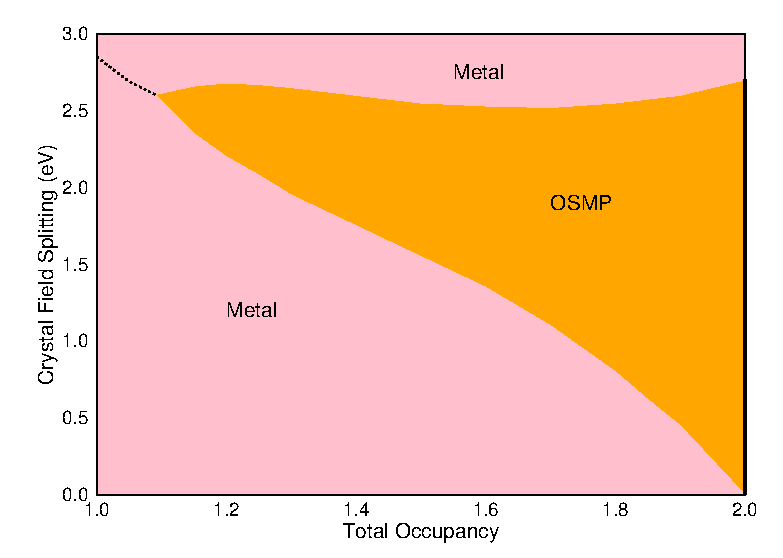
\includegraphics{figure/phase1.eps}
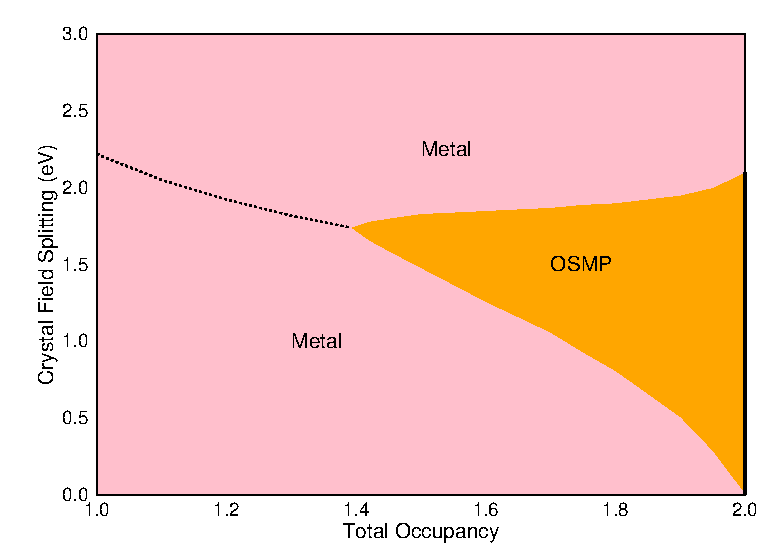
\includegraphics{figure/phase2.eps}
\caption[总占据数$N$与晶体场$\Delta$的相图]
        {总占据数$N$与晶体场$\Delta$的相图。上图:$U=4.90$\ eV,$J=0.25U$。
         下图:$U=4.90$\ eV,$J=0.20U$。在粉色区域里两个能带都是金属相;在橙
         色区域里能带2半满,处于Mott绝缘相,而能带1处于金属相。虚线代表能
         带2处于半满占据状态。} 
\label{fig:phase}
\end{figure}

\begin{figure}
\centering
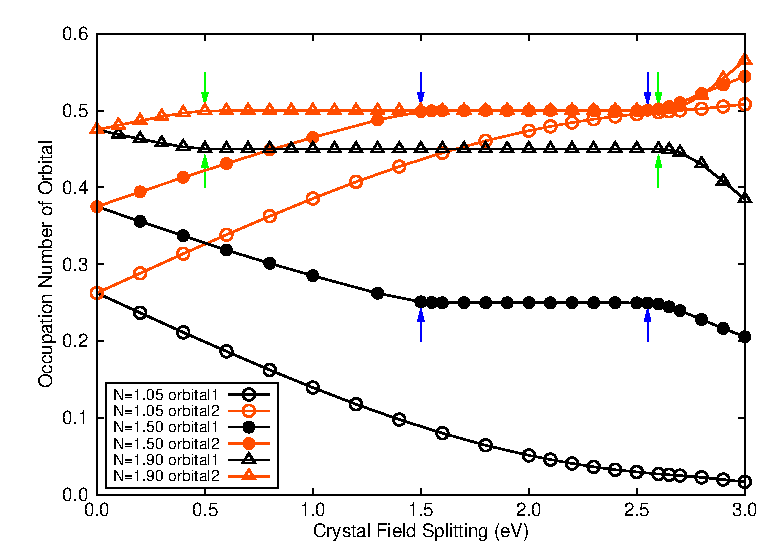
\includegraphics{figure/occu.eps}
\caption{能带的占据数随着晶体场变化的情况} 
\label{fig:occu}
\end{figure}

\begin{figure}
\centering
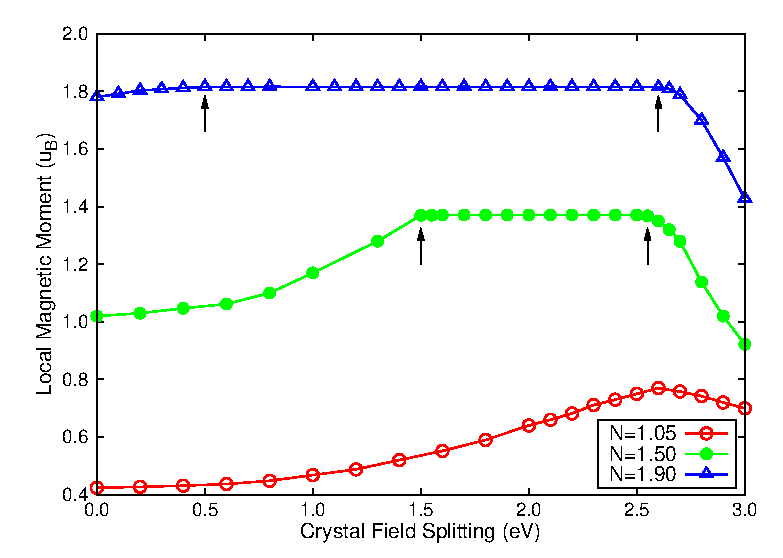
\includegraphics{figure/sz.eps}
\caption{局域磁矩随着晶体场变化的情况} 
\label{fig:magnetic}
\end{figure}

下面简单展示我们的计算结果。

图\ref{fig:phase}是关于总占据数$N$与晶体场劈裂
$\Delta$的相图,上图展示的是参数为$U=4.90$\ eV,$J=0.25U$的结果,下图展示的
是参数为$U=4.90$\ eV,$J=0.20U$的结果。从图中可以看出:当掺杂较小的时候,
两个能带都保持为金属相,即图中的粉色区域;当掺杂大于某个临界值时,能带2发生
金属$-$Mott绝缘体转变,而能带1依然保持为金属相,亦即此系统发生了具有轨道选
择性的金属$-$Mott绝缘体转变。如图中的橙色区域所示,我们称此区域为为具有轨道
选择性的Mott相(OSMP),掺杂越大OSMP区域将变得越大。对比上下两图可以发现,较
大的Hund交换作用$J$有利于形成OSMP。

图\ref{fig:occu}是固定总占据数$N$时各个能带占据数随着晶体场劈裂的变化情况。
从图中可以发现,进入OSMP区域后能带2的占据数为半满,剩下的电子占据能带1。

图\ref{fig:magnetic}是总占据数$N$固定时局域磁矩随着晶体场劈裂的变化情况。从
图中我们可以看出,较大的掺杂导致系统形成了较大的局域磁矩,而较大的局域磁矩的
存在是导致体系发生具有轨道选择性的Mott转变的根源。

\subsection{三带Anderson杂质模型中的轨道Kondo效应和自旋Kondo效应}

对于同时具有轨道磁矩和自旋磁矩的磁性杂质,多带Anderson杂质模型是一个很好的
模型。人们发现轨道Kondo效应和自旋Kondo效应在此模型中能同时存在\cite{werner:166405,yin:1206}。
在本小节中,我们将简单研究三带Anderson杂质模型中的轨道Kondo效应和自旋Kondo
效应。在该模型中,当平均电子数为$N=2$或者$4$时,系统具有$L=S=1$的总轨道和
自旋角动量。当温度降低时,轨道和自旋磁矩将渐渐地被bath里的自由电子屏蔽。我
们使用{\begonia}组件系统计算了该模型杂质部分的轨道磁化系数和自旋磁化系数。根
据这些磁化系数,我们发现轨道磁化和自旋磁化在温度降低时趋于饱和,发生Kondo转
变,并且轨道的Kondo温度比自旋的Kondo温度要高一个数量级。

1.\underline{模型哈密顿量}

该三带Anderson杂质模型的局域哈密顿量如下所示:
\begin{equation}
\begin{split}
H_{loc} = &- \sum_{a\sigma}(\mu - \Delta_a) n_{a\sigma} + \sum_{a} Un_{a\uparrow}n_{a\downarrow} \\
          &+ \sum_{a > b,\sigma}[U'n_{a\sigma}n_{b\bar{\sigma}} + (U'-J)n_{a\sigma}n_{b\sigma}] \\
          &- \sum_{a < b} J (d^{\dagger}_{a\downarrow}d^{\dagger}_{b\uparrow}d_{b\downarrow}d_{a\uparrow} 
           + d^{\dagger}_{b\uparrow}d^{\dagger}_{b\downarrow}d_{a\uparrow}d_{a\downarrow} + h.c.).
\end{split}
\end{equation}
其中,$a$,$b$为能带指标($a, b = 1 \sim 3$),$\sigma$为自旋指标,$n_{a\sigma} = 
c^{\dagger}_{a\sigma}c_{a\sigma}$为占据数算符,$\mu$为化学势,$\Delta$为杂
质能级\footnote{在本案例中$\Delta = 0$。}。$U$($U^{\prime}$)分别为轨道间
(轨道内)Coulomb相互作用,$J$为Hund交换相互作用,我们采取如下限制
$U=U^{\prime}+2J$。实际上,该局域哈密顿量与公式(\ref{eq:loc})中所描述的哈
密顿量基本一致,只是能带数目有所不同。

2.\underline{计算细节}

我们采用线性响应的方法来计算杂质部分的轨道磁化系数和自旋磁化系数,计算要点如下:
\begin{itemize}
  \item 半能带宽度$D= 2t=1.0$\ eV,三个能带完全简并
  \item Coulomb相互作用$U=5.0$\ eV,Hund交换相互作用$J = U/3$或者$U/6$
  \item 在局域部分哈密顿量加上Zeeman项:$H_{Z} = \mu_{B}H_{z}(\hat{L}_{z} + 2\hat{S}_{z})$
  \item 对角化原子问题,对于每个原子本征态$\Gamma$,给出总轨道角动量的$z$
        分量的平均值$L^{z,tot}_{\Gamma}$和总自旋角动量的$z$分量的平均
        值$S^{z,tot}_{\Gamma}$
  \item 使用{\begonia}组件进行单步计算,杂化函数由ctqmc程序初始化产生,不需要用
        户提供任何solver.hyb.in文件。计算得到原子组态概率$P_{\Gamma}$,则杂质部
        分的总轨道角动量的$z$分量的平均值为
        $L^{z}_{tot}=\sum_{\Gamma} P_{\Gamma} L^{z,tot}_{\Gamma}$,总自旋角动量
        的$z$分量的平均值为
        $S^{z}_{tot}=\sum_{\Gamma} P_{\Gamma} S^{z,tot}_{\Gamma}$
  \item 根据线性响应理论,轨道磁化系数为
        $\chi_{\text{orb}}=L^{z}_{tot}/H_{z}$,
        自旋磁化系数为
        $\chi_{\text{spin}}=S^{z}_{tot}/H_{z}$
\end{itemize}

3.\underline{计算结果及分析}

\begin{figure}
\centering
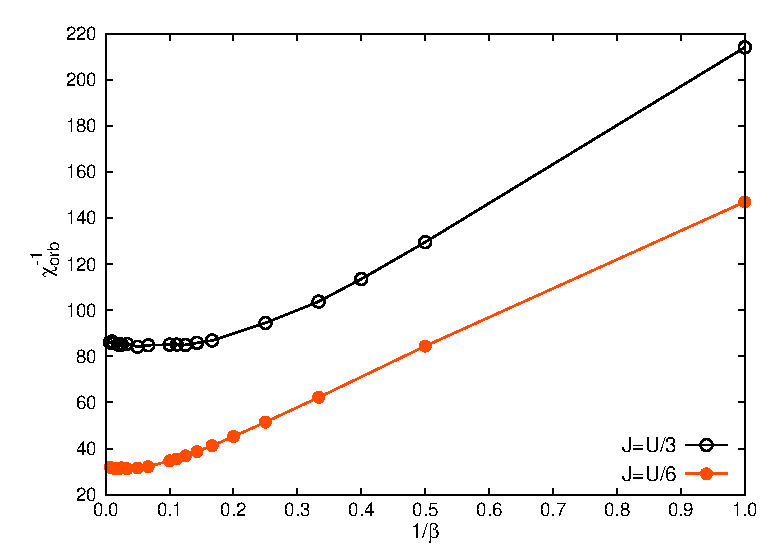
\includegraphics{figure/orb_chi.eps}
\caption{三带Anderson杂质模型中杂质的轨道磁化系数$\chi^{-1}_{\text{orb}}$随着温度的变化} 
\label{fig:orb_chi}
\end{figure}

\begin{figure}
\centering
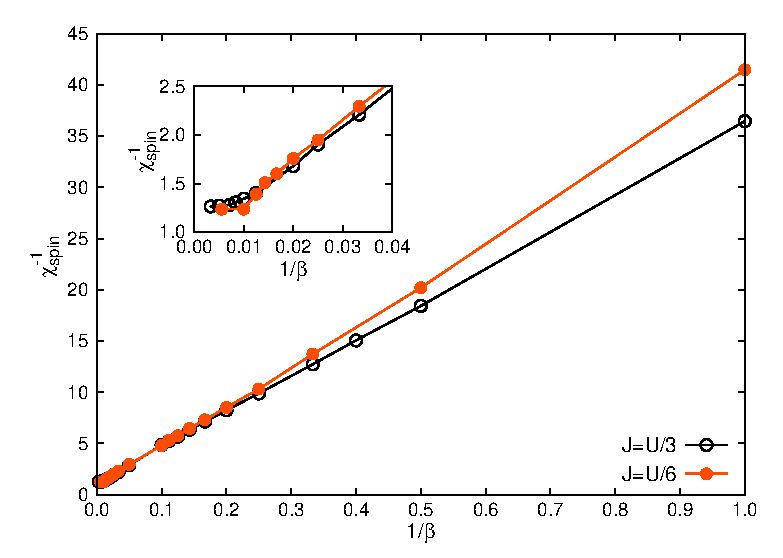
\includegraphics{figure/spin_chi.eps}
\caption{三带Anderson杂质模型中杂质的自旋磁化系数$\chi^{-1}_{\text{spin}}$随着温度的变化} 
\label{fig:spin_chi}
\end{figure}

下面简单展示我们的计算结果。图\ref{fig:orb_chi}是杂质的轨道磁化系数
$\chi^{-1}_{\text{orb}}$随着温度的变化,图\ref{fig:spin_chi}是杂质的
自旋磁化系数$\chi^{-1}_{\text{spin}}$随着温度的变化。从图中可以看出:
在温度较高时,磁化系数显示出居里$-$外斯的特征,表示系统具有自由的局
域磁矩存在;当温度降低时磁化趋于饱和,局域磁矩被屏蔽。Kondo温度定义为
磁矩被完全屏蔽的转变点,图\ref{fig:orb_chi}显示轨道部分的Kondo温度大
约为0.1\ eV,图\ref{fig:spin_chi}显示自旋部分的Kondo温度大约为0.01\ eV,
可见轨道Kondo温度比自旋Kondo温度约高一个数量级。
